% =====================================================================
%  Tesi magistrale in Scienze Statistiche
%  Effetto dei sistemi di accumulo a batteria sul Mercato del Giorno Prima del mercato elettrico italiano
% =====================================================================
\documentclass[12pt,a4paper,oneside]{report}

% --- Codifica e font ------------------------------------------------
% Ordine importante: fontenc/inputenc -> amsmath -> newtx.
% newtxtext+newtxmath forniscono un font "Times New Roman"-like,

\usepackage[T1]{fontenc}
\usepackage[utf8]{inputenc}

% --- Matematica  --------------------
\usepackage{amsmath}
\usepackage{amssymb}
\usepackage{amsthm}

% --- Font Times-like -------------------------------------------------
\usepackage{newtxtext,newtxmath}

% --- Lingua ----------------------------------------------------------
\usepackage[italian]{babel}
\usepackage{csquotes}          % richiesto da biblatex insieme a babel
\usepackage{textcomp}          % fornisce \texteuro (il comando \euro non esiste di base)
\usepackage{siunitx}           % per il comando \SI e le unità

% --- Figure, tabelle, impaginazione ----------------------------------
\usepackage{graphicx}
\graphicspath{{figure/}{../output/figure/}}
\usepackage{booktabs}
\usepackage{float}
\usepackage{caption}
\usepackage[printonlyused]{acronym} % printonlyused: mostra solo gli acronimi citati

% --- Margini: 2,5 cm sopra/sotto; 3 cm ai lati (range 2,5/3) ---------
\usepackage[a4paper,top=2.5cm,bottom=2.5cm,left=3cm,right=3cm]{geometry}

% --- Interlinea 1,5 --------------------------------------------------
\usepackage{setspace}
\onehalfspacing

% --- Rientro prima riga di OGNI paragrafo, 1,5 cm --------------------
% indentfirst forza il rientro anche sul primo paragrafo dopo un titolo.

\usepackage{indentfirst}
\setlength{\parindent}{1.5cm}

% --- Dimensioni titoli: section 16pt, subsection 14pt ---------------
\usepackage{titlesec}
\titleformat{\section}
  {\normalfont\fontsize{16pt}{19pt}\bfseries}{\thesection}{1em}{}
\titleformat{\subsection}
  {\normalfont\fontsize{14pt}{17pt}\bfseries}{\thesubsection}{1em}{}

% --- Codice sorgente -------------------------------------------------
\usepackage{xcolor}
\usepackage{listings}

\definecolor{grigioChiaro}{gray}{0.95}
\definecolor{verdeCommento}{rgb}{0.0,0.45,0.2}
\definecolor{bluParola}{rgb}{0.1,0.1,0.6}
\definecolor{rossoStringa}{rgb}{0.6,0.1,0.1}

\lstset{
  language=Python,
  basicstyle=\ttfamily\footnotesize,
  keywordstyle=\color{bluParola}\bfseries,
  commentstyle=\color{verdeCommento}\itshape,
  stringstyle=\color{rossoStringa},
  backgroundcolor=\color{grigioChiaro},
  numbers=left,
  numberstyle=\tiny\color{gray},
  numbersep=8pt,
  frame=single,
  rulecolor=\color{gray},
  breaklines=true,
  breakatwhitespace=true,
  showstringspaces=false,
  columns=flexible,
  captionpos=b,
  extendedchars=true,
  % Le lettere accentate dentro i listati vanno dichiarate esplicitamente,
  % altrimenti listings non le sa rappresentare.
  literate=%
    {à}{{\`a}}1 {è}{{\`e}}1 {é}{{\'e}}1 {ì}{{\`i}}1 {ò}{{\`o}}1 {ù}{{\`u}}1
    {À}{{\`A}}1 {È}{{\`E}}1 {É}{{\'E}}1 {Ì}{{\`I}}1 {Ò}{{\`O}}1 {Ù}{{\`U}}1
    {€}{{\texteuro{}}}1
}
\renewcommand{\lstlistingname}{Codice}
\renewcommand{\lstlistlistingname}{Elenco dei codici}

% --- Bibliografia ----------------------------------------------------
% Se biber non fosse disponibile, sostituire con:
%   \usepackage[backend=bibtex,style=numeric,sorting=nyt]{biblatex}
\usepackage[backend=biber,style=numeric,sorting=none]{biblatex}
\addbibresource{bibliografia.bib}

% --- Collegamenti ipertestuali --------------
\usepackage[hidelinks]{hyperref}

% --- Comandi di comodo -----------------------------------------------
\newcommand{\eur}{\texteuro}
\newcommand{\euromwh}{\texteuro/MWh}
\newcommand{\mgp}{MGP}
\newcommand{\bess}{BESS}

\begin{document}

% =====================================================================
%  FRONTESPIZIO 
% =====================================================================
\begin{titlepage}
\centering

{\large UNIVERSIT\`A DEGLI STUDI DI MILANO-BICOCCA\par}
\vspace{0.1cm}
{\large Scuola di Economia e Statistica\par}
\vspace{0.3cm}
{\large Corso di Laurea Magistrale in  \\ SCIENZE STATISTICHE ED ECONOMICHE\par}

\vskip 1cm
\begin{center}
    
\includegraphics[height=3.2cm]{figure/logo-unimib.png}
\end{center}

\vfill

{\Huge\bfseries Effetto dei sistemi di accumulo a batteria sul Mercato del Giorno Prima del mercato elettrico italiano\par}
\vspace{1cm}
{\Large\itshape [Eventuale sottotitolo]\par}

\vfill

\begin{flushleft}
\begin{tabular}{@{}ll@{}}
\textbf{Relatore:}    & Prof. Matteo Pelagatti \\[0.3cm]
\textbf{Correlatore:} & Prof.  \\
\end{tabular}
\end{flushleft}

\vspace{1cm}

\begin{flushright}
\begin{tabular}{@{}ll@{}}
\textbf{Tesi di laurea di:} & Enrico Sterza \\
\textbf{Matr. N.} & 874099\\
\end{tabular}
\end{flushright}

\vfill

{\large Anno Accademico 2025/2026\par}

\end{titlepage}

% --- Pagina vuota dopo il frontespizio --------------------------------
\clearpage
\thispagestyle{empty}
\null
\clearpage

% --- Ringraziamenti ---
% --- citazione --------------------------------
\begin{flushright}
{ \textit{I did stop believing it a lot of times. \\ But the next day I always woke up and fought for it again.} \\
\vspace{10pt}
Wout Van Aert, post vittoria Paris-Roubaix 2026
}
\end{flushright}

\vspace{13pt}

Some acknowledgments to family, friends, supervisors, etc.

\thispagestyle{empty}
\mbox{}
\newpage
\clearpage

% --- Abstract ---
\chapter*{Abstract}


Qui inserire testo


\thispagestyle{empty}
\mbox{}
\newpage
\clearpage

% =====================================================================
%  INDICI
% =====================================================================
\pagenumbering{roman}

\tableofcontents
\clearpage

% --- Elenco delle Figure ---
\phantomsection
\addcontentsline{toc}{chapter}{\listfigurename} % Aggiunge "Elenco delle figure" all'indice
\listoffigures
\clearpage

\chapter*{Elenco degli acronimi}
\phantomsection
\addcontentsline{toc}{chapter}{Elenco degli acronimi}
\markboth{Elenco degli acronimi}{Elenco degli acronimi}

\begin{acronym}[DDS 2024] % Il parametro tra quadre definisce la larghezza della colonna (inserire l'acronimo più lungo)
\acro{PNIEC}{Piano Nazionale Integrato Energia e Clima}
\acro{FRNP}{Fonti Rinnovabili Non Programmabili}
\acro{GME}{Gestore dei Mercati Energetici}
\acro{RTN}{Rete di Trasmissione Nazionale}
\acro{DDS 2024}{Documento di Descrizione degli Scenari 2024}
\acro{MACSE}{Meccanismo di Approvvigionamento di Capacità di Stoccaggio Elettrico}
\acro{FER}{Fonti di Energia Rinnovabile}
  \acro{BESS}{Battery Energy Storage System}
  \acro{MGP}{Mercato del Giorno Prima}
  \acro{MPEG}{Mercato dei Prodotti Giornalieri}
  \acro{MI}{Mercati Infragiornalieri}
  \acro{MSD}{Mercato per il Servizio di Dispacciamento}
  \acro{MBR}{Mercato per il Bilanciamento e il Ridispacciamento}
\acro{TSO}{Transmission System Operator}
\acro{DSO}{Distribution System Operator}
\acro{MPE}{Mercato Elettrico a Pronti}
\acro{SDAC}{Single Day-Ahead Coupling}
\acro{PCR}{Price Coupling of Regions }
\acro{MILP}{Mixed-Integer Linear Programming}
\acro{MTU}{Market Time Unit}
\acro{PUN}{Prezzo Unico Nazionale}
\acro{XML}{eXtensible Markup Language}
\acro{SdS}{Sistemi di Stoccaggio}
\acro{RTE}{Round-Trip Efficiency}
\end{acronym}
\clearpage

\pagenumbering{arabic}



% =====================================================================
%  CAPITOLI
% =====================================================================
\chapter{Introduzione e Contesto}
\label{cap:introduzione}

% DA COMPLETARE: capitolo introduttivo. Le sezioni 1.1-1.3 richiedono fonti esterne
% (dati Terna e ARERA sulla capacita' rinnovabile installata, documentazione MACSE sulle
% aste per la capacita' di accumulo, letteratura sull'arbitraggio con storage).
% La sezione 1.4 va scritta per ultima, quando gli obiettivi saranno stabilizzati.

\section{La transizione energetica in Italia}
\label{sec:transizione}

% DA COMPLETARE: inquadramento del contesto.
% Elementi da trattare, con dati da reperire e citare:
%   - crescita della capacita' rinnovabile non programmabile (fotovoltaico ed eolico)
%     in Italia negli ultimi anni;
%   - effetto sui prezzi di mercato: compressione dei prezzi diurni, aumento della
%     volatilita' infragiornaliera, comparsa di prezzi negativi;
%   - obiettivi al 2030 del PNIEC e fabbisogno di flessibilita' stimato da Terna.

Il sistema elettrico italiano sta attraversando una fase di trasformazione profonda, guidata
dalla penetrazione crescente di fonti rinnovabili non programmabili. L'effetto di questa
trasformazione sul mercato non riguarda soltanto il livello medio dei prezzi, ma soprattutto
la loro \emph{forma} nell'arco della giornata: la produzione fotovoltaica comprime i prezzi
nelle ore centrali e li lascia elevati nelle ore serali, quando la domanda resta alta e
l'irraggiamento e' venuto meno.

\`E proprio questo divario infragiornaliero a costituire l'opportunit\`a economica per i
sistemi di accumulo, ed \`e la grandezza su cui si concentra il presente lavoro.

\section{I sistemi di accumulo a batteria (BESS)}
\label{sec:bess}

% DA COMPLETARE: descrizione tecnologica ed economica dei BESS.
% Elementi da trattare:
%   - principio di funzionamento e grandezze caratteristiche: potenza nominale (MW),
%     capacita' energetica (MWh), rapporto energia/potenza (durata), efficienza di
%     ciclo completo (round-trip), profondita' di scarica;
%   - servizi che un BESS puo' fornire: arbitraggio sui mercati dell'energia, riserva,
%     regolazione di frequenza, capacity market;
%   - stato dell'arte in Italia: capacita' installata, aste MACSE, prospettive.

\section{Il quesito degli investitori}
\label{sec:quesito}

% DA COMPLETARE: impostazione della domanda di ricerca dal punto di vista dell'investitore.
% Il punto centrale, che il lavoro svolto permette gia' di argomentare, e' il seguente:
% la redditivita' di un impianto di accumulo dipende dal differenziale di prezzo fra ore
% di carica e ore di scarica, ma quel differenziale non e' un dato esogeno: l'accumulo,
% comprando nelle ore basse e vendendo nelle ore alte, riduce esso stesso il differenziale
% da cui trae profitto. Questo effetto di retroazione e' il cuore metodologico della tesi.

\section{Obiettivi della tesi}
\label{sec:obiettivi}

% DA COMPLETARE: da rifinire quando i risultati saranno consolidati.
% Formulazione provvisoria degli obiettivi, coerente con il lavoro svolto finora.

Il lavoro si propone tre obiettivi.

Il primo \`e \textbf{ricostruire il meccanismo di formazione del prezzo} sul Mercato del
Giorno Prima a partire dai dati pubblici delle offerte, in modo da poter calcolare non solo
il prezzo osservato ma anche il prezzo \emph{controfattuale} che si sarebbe formato in
presenza di capacit\`a di accumulo. Questo obiettivo \`e stato raggiunto ed \`e documentato
nel Capitolo~\ref{cap:simulazione}.

Il secondo \`e \textbf{simulare l'effetto di quantit\`a crescenti di accumulo} sui prezzi e
sulle quantit\`a di equilibrio della zona NORD, tenendo conto dell'effetto di retroazione che
l'accumulo stesso esercita sul prezzo.

Il terzo \`e \textbf{determinare il dimensionamento ottimale} dell'accumulo — capacit\`a
energetica, potenza e durata di carica e scarica — e valutarne la redditivit\`a dal punto di
vista di un investitore.

\section{Organizzazione del documento}
\label{sec:organizzazione}

Il Capitolo~\ref{cap:mercato} descrive l'architettura del mercato elettrico italiano e i
meccanismi d'asta rilevanti per il lavoro. Il Capitolo~\ref{cap:strategia} formula il
problema di ottimizzazione della strategia di accumulo. Il Capitolo~\ref{cap:simulazione}
presenta i dati, la ricostruzione delle curve di domanda e offerta e la sua validazione. Il
Capitolo~\ref{cap:valutazione} traduce i risultati in termini economici e finanziari. Il
Capitolo~\ref{cap:conclusioni} riassume i risultati e ne discute i limiti.

\subsection{Citations}
\label{sec:citations}

% DA COMPLETARE: sostituire con le convenzioni effettivamente adottate.

I riferimenti bibliografici sono gestiti con \texttt{biblatex} in stile numerico e sono
raccolti nel file \texttt{bibliografia.bib}. Nel testo una citazione appare come
\texttt{\textbackslash cite\{chiave\}}; le fonti dei dati di mercato sono citate per esteso
alla prima occorrenza.

\subsection{Use of acronyms}
\label{sec:acronimi}

% DA COMPLETARE: valutare se introdurre il pacchetto acronym o glossaries per generare
% automaticamente l'elenco degli acronimi. Per ora l'elenco e' compilato a mano.

Gli acronimi sono definiti per esteso alla prima occorrenza e usati in forma abbreviata nel
seguito. I principali sono riportati nella Tabella~\ref{tab:acronimi}.

\begin{table}[H]
\centering
\caption{Acronimi ricorrenti nel documento.}
\label{tab:acronimi}
\begin{tabular}{@{}ll@{}}
\toprule
\textbf{Sigla} & \textbf{Significato} \\
\midrule
BESS   & \emph{Battery Energy Storage System}, sistema di accumulo a batteria \\
GME    & Gestore dei Mercati Energetici \\
MGP    & Mercato del Giorno Prima \\
MI     & Mercati Infragiornalieri \\
MSD    & Mercato per il Servizio di Dispacciamento \\
MTU    & \emph{Market Time Unit}, periodo elementare di mercato \\
PUN    & Prezzo Unico Nazionale \\
XML    & \emph{eXtensible Markup Language}, formato dei dati pubblicati dal GME \\
\bottomrule
\end{tabular}
\end{table}

\chapter{Il Mercato Elettrico Italiano}
\label{cap:mercato}

Questo capitolo descrive l'architettura del mercato elettrico italiano limitatamente a
quanto serve per il lavoro: la struttura delle sedi di negoziazione, il funzionamento
dell'asta del Mercato del Giorno Prima e la natura della variabilit\`a dei prezzi. La
descrizione del MGP \`e basata sui dati effettivamente utilizzati, le cui caratteristiche
sono documentate nel Capitolo~\ref{cap:simulazione}.

\section{Struttura del GME (Gestore dei Mercati Energetici)}
\label{sec:gme}

Il Gestore dei Mercati Energetici (GME) organizza le sedi di negoziazione dell'energia
elettrica all'ingrosso in Italia. Ai fini di questo lavoro rilevano tre caratteristiche
della sua architettura.

La prima \`e la \textbf{sequenzialit\`a} delle sedi: il Mercato del Giorno Prima si chiude
prima dei Mercati Infragiornalieri, che a loro volta precedono il Mercato per il Servizio di
Dispacciamento. Un operatore che modifica la propria posizione lo fa quindi in momenti
successivi e con informazioni via via pi\`u precise.

La seconda \`e la \textbf{zonalit\`a}: il territorio nazionale \`e suddiviso in zone di
mercato, ciascuna con un proprio prezzo quando i limiti di transito fra zone sono
vincolanti. Nel giorno pilota analizzato compaiono sette zone fisiche italiane — NORD, CNOR,
CSUD, SUD, CALA, SICI, SARD — accanto a zone \emph{virtuali} che rappresentano le frontiere
con l'estero.

La terza \`e la \textbf{trasparenza dei dati}: il GME pubblica, per ciascun giorno e per
ciascuna sede, l'insieme completo delle offerte presentate, comprese quelle rifiutate. \`E
questa disponibilit\`a che rende possibile la ricostruzione delle curve aggregate su cui si
fonda l'intero lavoro: senza il dettaglio delle offerte non accettate la curva sarebbe
troncata proprio nel punto che interessa, cio\`e attorno all'equilibrio.

\section{MGP e MI (Mercato del Giorno Prima e Mercati Infragiornalieri)}
\label{sec:mgp}

\subsection*{Il meccanismo d'asta}

Il Mercato del Giorno Prima \`e un'\textbf{asta a prezzo uniforme}: gli operatori presentano
coppie prezzo--quantit\`a, distinte fra acquisto e vendita, riferite a un singolo periodo e a
una singola zona. L'algoritmo di mercato ordina le offerte di vendita per prezzo crescente e
quelle di acquisto per prezzo decrescente, ottenendo due funzioni a gradini, e ne individua
l'intersezione. Tutte le offerte accettate sono remunerate al medesimo prezzo, quello di
equilibrio, indipendentemente dal prezzo a cui erano state presentate.

Formalmente, indicando con $S(p)$ la quantit\`a complessivamente offerta in vendita a un
prezzo non superiore a $p$ e con $D(p)$ quella domandata a un prezzo non inferiore a $p$, il
prezzo di equilibrio \`e
\begin{equation}
p^{*} \;=\; \min \{\, p \;:\; S(p) \ge D(p) \,\}.
\label{eq:clearing}
\end{equation}

La funzione $S$ \`e non decrescente e la funzione $D$ non crescente, quindi l'eccesso di
offerta $S(p) - D(p)$ \`e monotono non decrescente e l'insieme dei prezzi che pareggiano il
mercato \`e sempre una semiretta: il prezzo di equilibrio ne \`e l'estremo inferiore. Quando
l'eccesso si annulla su un intervallo di prezzi l'equilibrio non \`e unico e la scelta del
punto diventa una convenzione; sui dati esaminati questo accade nello 0{,}8\% delle aste
orarie e in nessuna di quelle a quarto d'ora, quindi non costituisce una fonte rilevante di
ambiguit\`a.

\subsection*{Il periodo di mercato}

Il periodo elementare d'asta (\emph{Market Time Unit}) \`e cambiato durante il periodo
coperto dai dati. Fino al 30 settembre 2025 il mercato era organizzato su base
\textbf{oraria}, con ventiquattro aste indipendenti al giorno; dal 1\textsuperscript{o}
ottobre 2025 \`e passato al \textbf{quarto d'ora}, con novantasei aste al giorno. Il
passaggio \`e netto e verificabile nei dati: il 30 settembre 2025 la totalit\`a delle offerte
\`e oraria, il giorno successivo l'82{,}8\% \`e a quarto d'ora.

Questa discontinuit\`a ha conseguenze dirette sul disegno dello studio, discusse nella
Sezione~\ref{sec:dataset}: l'anno solare 2025 non \`e omogeneo, e la risoluzione temporale
non \`e neutrale per la valutazione di una strategia di arbitraggio, che dipende da quanto
\`e fine la griglia su cui l'accumulo pu\`o caricare e scaricare.

\subsection*{Tipologie di offerta}

Accanto alle offerte \emph{semplici}, riferite a un singolo periodo e frazionabili, esistono
le \textbf{offerte a blocchi}, accettabili solo per intero e su tutti i periodi che coprono.
Sui dati esaminati un blocco copre da quattro a novantasei periodi, ha un prezzo unico e uno
stato identico in tutti i suoi periodi: non si osserva alcun blocco accettato soltanto su una
parte di essi.

La presenza di offerte a blocchi rende il problema d'asta un programma con vincoli di
interezza e genera il fenomeno del \emph{rifiuto paradossale}: un blocco pu\`o risultare in
merito sul prezzo e venire comunque respinto, perch\'e accettarlo renderebbe inconsistente la
soluzione. I dati riportano questi casi con un codice di stato dedicato.

\subsection*{I Mercati Infragiornalieri}

% DA COMPLETARE: descrizione dei MI, da sviluppare se l'analisi verra' estesa oltre il MGP.
% Elementi da trattare: sessioni ad asta MI-A1/A2/A3, negoziazione continua XBID, funzione
% di aggiustamento delle posizioni assunte sul MGP, e implicazioni per un accumulo che
% volesse operare anche su queste sedi.

\section{MSD (Mercato per il Servizio di Dispacciamento)}
\label{sec:msd}

% DA COMPLETARE: descrizione del MSD.
% Elementi da trattare:
%   - finalita': approvvigionamento delle risorse per il bilanciamento in tempo reale
%     e per la risoluzione delle congestioni, con Terna come controparte unica;
%   - meccanismo pay-as-bid, diverso dal prezzo uniforme del MGP;
%   - rilevanza per un BESS: i ricavi da MSD sono spesso superiori a quelli da arbitraggio
%     sul MGP, quindi ignorarli sottostima la redditivita' complessiva dell'investimento.
%     Questa esclusione va dichiarata fra i limiti del modello (Sezione 6.2).

\section{L'aleatorietà del prezzo}
\label{sec:aleatorieta}

Il prezzo zonale \`e la variabile aleatoria centrale del problema. Due sue caratteristiche
sono direttamente rilevanti per la strategia di accumulo.

\paragraph{Ampiezza dell'escursione infragiornaliera.} \`E il differenziale fra ore a prezzo
basso e ore di picco, cio\`e esattamente il margine lordo di un ciclo di arbitraggio. Nel
mese di gennaio 2025 il prezzo zonale della zona NORD si \`e mosso fra un minimo orario medio
di circa 116~\euromwh{} nelle ore notturne e un massimo di circa 172~\euromwh{} nelle ore di
picco serale.

\paragraph{Limiti di prezzo e prezzi negativi.} I prezzi ammessi sul mercato non sono
confinati ai valori positivi: sui dati esaminati le offerte spaziano da $-500$ a
$4\,000$~\euromwh{}. La possibilit\`a di prezzi negativi \`e caratteristica dei sistemi ad
alta penetrazione rinnovabile, dove in alcune ore conviene pagare per immettere energia
piuttosto che modulare la produzione, ed \`e proprio la condizione in cui l'accumulo trova le
occasioni di acquisto pi\`u convenienti.

\paragraph{Rigidit\`a della domanda.} Una quota rilevante della domanda \`e presentata al
prezzo massimo, cio\`e \`e disposta ad acquistare a qualunque prezzo: nel giorno pilota si
tratta del 52\% delle offerte di acquisto della zona NORD. La curva di domanda risulta quindi
molto ripida e l'effetto di un accumulo sul prezzo passa quasi interamente attraverso la
curva di offerta. \`E un elemento da tenere presente nell'interpretazione degli scenari del
Capitolo~\ref{cap:simulazione}.

% DA COMPLETARE: analisi statistica della serie dei prezzi (stagionalita' settimanale e
% annuale, persistenza, distribuzione dell'escursione giornaliera). Da sviluppare quando
% sara' disponibile la ricostruzione su tutto l'anno 2025.

\chapter{Formulazione Teorica della Strategia Ottima}
\label{cap:strategia}

Questo capitolo formalizza il problema decisionale dell'operatore di un sistema di accumulo
che opera sul Mercato del Giorno Prima. La formulazione della funzione obiettivo e del
modello fisico \`e impostata; il modello di degrado e la gestione dell'incertezza sono
ancora da sviluppare.

\section{Definizione della Funzione Obiettivo}
\label{sec:obiettivo}

\subsection*{Notazione}

Si consideri una giornata suddivisa in $T$ periodi di mercato indicizzati da
$t = 1, \dots, T$, ciascuno di durata $\Delta_t$ ore ($\Delta_t = 1$ per le aste orarie,
$\Delta_t = 0{,}25$ per quelle a quarto d'ora). Per ogni periodo si definiscono:

\begin{itemize}
  \item $c_t \ge 0$: potenza assorbita in carica nel periodo $t$, in MW;
  \item $s_t \ge 0$: potenza immessa in scarica nel periodo $t$, in MW;
  \item $e_t$: energia immagazzinata alla fine del periodo $t$, in MWh;
  \item $p_t$: prezzo di equilibrio del periodo $t$, in \euromwh{}.
\end{itemize}

\subsection*{Il ricavo e l'effetto di retroazione}

Se l'accumulo fosse di taglia trascurabile rispetto al mercato, il prezzo sarebbe un dato
esogeno e il ricavo giornaliero si scriverebbe semplicemente come
\begin{equation}
\Pi^{\text{price taker}} \;=\; \sum_{t=1}^{T} p_t \,\Delta_t \,(s_t - c_t).
\label{eq:ricavo-pricetaker}
\end{equation}

Questa formulazione, per\`o, ignora il meccanismo che costituisce l'oggetto della tesi: un
accumulo che carica aggiunge domanda e fa \emph{salire} il prezzo, e che scarica aggiunge
offerta e lo fa \emph{scendere}. Il prezzo non \`e quindi un dato ma una funzione della
decisione stessa:
\begin{equation}
p_t \;=\; \pi_t\!\left(c_t, s_t\right),
\label{eq:prezzo-endogeno}
\end{equation}
dove $\pi_t$ \`e la funzione che restituisce il prezzo di equilibrio del periodo $t$ dopo
aver inserito nelle curve d'asta la domanda addizionale $c_t$ e l'offerta addizionale $s_t$.
Questa funzione non ha forma analitica chiusa: \`e definita dall'algoritmo di
clearing~\eqref{eq:clearing} applicato alle curve ricostruite dai dati, ed \`e implementata
nel modulo descritto nella Sezione~\ref{sec:setup}.

Il problema dell'operatore diventa quindi
\begin{equation}
\max_{\{c_t,\, s_t\}} \quad
\Pi \;=\; \sum_{t=1}^{T} \pi_t\!\left(c_t, s_t\right) \Delta_t \left(s_t - c_t\right)
\;-\; \Phi\!\left(\{c_t, s_t\}\right),
\label{eq:obiettivo}
\end{equation}
dove $\Phi$ rappresenta il costo di degrado associato al profilo di utilizzo
(Sezione~\ref{sec:degrado}).

\paragraph{Osservazione.} La retroazione agisce \emph{contro} l'operatore in entrambe le
direzioni: comprando fa salire il prezzo di acquisto, vendendo fa scendere quello di vendita.
Il margine di arbitraggio si riduce quindi al crescere della taglia dell'accumulo, ed \`e
questo il meccanismo che rende il dimensionamento un problema non banale — al di sopra di una
certa capacit\`a, l'accumulo distrugge da s\'e la propria fonte di reddito. La misura di
questo effetto \`e riportata nella Sezione~\ref{sec:esecuzione}.

\section{Modello fisico della batteria}
\label{sec:modello-fisico}

Il bilancio energetico dell'accumulo lega lo stato di carica fra periodi consecutivi:
\begin{equation}
e_t \;=\; e_{t-1} \;+\; \eta^{c}\, c_t\, \Delta_t \;-\; \frac{s_t\, \Delta_t}{\eta^{s}},
\qquad t = 1, \dots, T,
\label{eq:bilancio}
\end{equation}
dove $\eta^{c}$ ed $\eta^{s}$ sono i rendimenti di carica e di scarica; il loro prodotto
$\eta = \eta^{c}\eta^{s}$ \`e il rendimento di ciclo completo.

Il problema \`e soggetto ai vincoli
\begin{align}
0 \;\le\; e_t \;&\le\; E^{\max}, \label{eq:vincolo-energia}\\
0 \;\le\; c_t \;&\le\; P^{\max}, \label{eq:vincolo-carica}\\
0 \;\le\; s_t \;&\le\; P^{\max}, \label{eq:vincolo-scarica}\\
c_t \cdot s_t \;&=\; 0, \label{eq:vincolo-esclusione}
\end{align}
dove $E^{\max}$ \`e la capacit\`a energetica in MWh e $P^{\max}$ la potenza nominale in MW.
Il loro rapporto $E^{\max}/P^{\max}$ \`e la \emph{durata} dell'accumulo, espressa in ore, ed
\`e uno dei parametri di dimensionamento che la tesi si propone di ottimizzare.

Il vincolo~\eqref{eq:vincolo-esclusione} impedisce di caricare e scaricare simultaneamente.
\`E un vincolo di complementarit\`a, non lineare; nella pratica pu\`o essere omesso quando i
prezzi sono positivi, perch\'e caricare e scaricare nello stesso periodo sarebbe comunque
non conveniente, ma va reintrodotto in presenza di prezzi negativi, che sui dati esaminati
sono ammessi fino a $-500$~\euromwh{}.

% DA COMPLETARE: scelta dei valori dei parametri fisici.
% Da fissare, con riferimento a fonti tecniche: rendimento di ciclo completo (tipicamente
% 0,85-0,92 per batterie agli ioni di litio), profondita' di scarica ammessa, eventuali
% vincoli di rampa, autoscarica. Va inoltre deciso se imporre e_T = e_0 (ciclo giornaliero
% chiuso), scelta che semplifica il confronto fra giornate.

\section{Modellazione del degrado}
\label{sec:degrado}

% DA COMPLETARE: modello di degrado della batteria.
% Elementi da trattare:
%   - distinzione fra degrado calendariale (funzione del tempo e dello stato di carica
%     medio) e degrado ciclico (funzione del numero e della profondita' dei cicli);
%   - scelta di una formulazione trattabile: costo marginale costante per MWh ciclato,
%     oppure conteggio dei cicli equivalenti con metodo rainflow;
%   - traduzione del degrado in un costo monetario Phi da inserire nella funzione
%     obiettivo (eq. 3.4), tipicamente come costo di sostituzione ripartito sui cicli
%     di vita utile;
%   - implicazione economica: il degrado introduce un costo opportunita' che rende non
%     conveniente ogni arbitraggio il cui differenziale di prezzo non lo copra, e quindi
%     riduce il numero di cicli ottimali rispetto al caso senza degrado.

\section{Gestione dell'incertezza}
\label{sec:incertezza}

% DA COMPLETARE: trattamento dell'incertezza sui prezzi.
% Il punto di partenza e' che la strategia ottimizzata sui prezzi realizzati costituisce
% un limite superiore irraggiungibile (perfect foresight): serve come termine di confronto,
% non come strategia realistica.
% Elementi da trattare:
%   - quantificazione del divario fra strategia con previsione perfetta e strategie
%     realizzabili sulla base dell'informazione disponibile alla chiusura del MGP;
%   - possibili impostazioni: ottimizzazione stocastica su scenari di prezzo, oppure
%     regole di decisione basate su previsioni puntuali con analisi dell'errore;
%   - collegamento con la Sezione 2.4 sull'aleatorieta' del prezzo.

\chapter{Simulazione e Analisi Pratica}
\label{cap:simulazione}

Questo capitolo descrive la parte operativa del lavoro: come sono stati trattati i dati
pubblici del GME, come sono state ricostruite le curve di domanda e offerta, e con quale
accuratezza la ricostruzione riproduce i prezzi effettivamente formatisi sul mercato. La
validazione \`e presentata prima degli scenari di accumulo perch\'e ne costituisce il
presupposto: un modello che non sa riprodurre il prezzo osservato non pu\`o essere usato per
calcolare un prezzo controfattuale.

\section{Setup della simulazione}
\label{sec:setup}

\subsection{Ricostruzione delle curve aggregate}

Per ogni asta — individuata da una zona e da un periodo — le offerte di vendita sono ordinate
per prezzo crescente e quelle di acquisto per prezzo decrescente, e le rispettive quantit\`a
sono cumulate. Si ottengono cos\`i le due funzioni a gradini $S(p)$ e $D(p)$ introdotte nella
Sezione~\ref{sec:mgp}, il cui punto di incontro definisce il prezzo di
equilibrio~\eqref{eq:clearing}.

Una precisazione sul perch\'e le curve siano costruite dalle \textbf{offerte} e non dal merit
order degli impianti. L'alternativa naturale sarebbe ordinare il parco di generazione per costo
marginale crescente, ricavandolo da combustibile, rendimento e costi della CO\textsubscript{2}.
\textcite{veenstra2025profitability} argomentano per\`o che sul breve periodo la relazione fra il
merit order costruito sugli impianti e le offerte effettivamente presentate al mercato \`e
\textbf{debole}, perch\'e un'offerta non corrisponde necessariamente a uno specifico impianto:
gli operatori presentano portafogli, aggregano capacit\`a in impianti virtuali e rivendono
energia acquistata altrove.

Ne segue che il merit order tecnico descrive il sistema fisico ma non la curva su cui il prezzo
si forma davvero. Poich\'e l'oggetto di questa tesi \`e precisamente \textbf{come l'accumulo
sposta il prezzo di equilibrio}, la rappresentazione pertinente \`e quella delle offerte, che
\`e anche l'unica osservabile senza stimare parametri di costo non pubblici. La scelta ha un
costo — le curve ricostruite non dicono nulla sulla tecnologia marginale — ma \`e quello giusto
da pagare per la domanda posta.

L'implementazione valuta le curve sull'insieme di tutti i prezzi presenti nell'asta.
L'insieme \`e sufficiente perch\'e le curve sono costanti a tratti e cambiano valore solo in
corrispondenza di un prezzo offerto: l'intersezione cade quindi sempre su uno di questi
punti. Il costo computazionale \`e $O(n \log n)$ nel numero $n$ di offerte del periodo,
dell'ordine del migliaio, il che rende praticabile l'esecuzione su decine di migliaia di
aste.

\begin{lstlisting}[caption={Ricerca del prezzo di equilibrio (\texttt{src/mgp/curve.py}).},
                   label={lst:clearing}]
def prezzo_equilibrio(offerte):
    """Il prezzo di equilibrio e' il piu' piccolo prezzo al quale l'offerta
    cumulata raggiunge la domanda cumulata: p* = min { p : S(p) >= D(p) }."""
    vendita  = offerte[offerte["PURPOSE_CD"] == "OFF"]
    acquisto = offerte[offerte["PURPOSE_CD"] == "BID"]
    if vendita.empty or acquisto.empty:
        return Equilibrio(None, None, None, None, "curva_vuota")

    # Le curve sono costanti a tratti: cambiano valore solo su un prezzo
    # offerto, quindi l'intersezione cade sempre su uno di questi punti.
    prezzi = np.unique(np.concatenate([p_off, p_dom]))
    S = offerta_cumulata_fino_a(prezzi)     # non decrescente
    D = domanda_cumulata_oltre(prezzi)      # non crescente

    incrocio = np.flatnonzero(S >= D)
    if incrocio.size == 0:
        return Equilibrio(None, None, None, None, "domanda_sempre_superiore")

    i = incrocio[0]
    # L'offerta marginale entra solo per la parte che pareggia la domanda.
    return Equilibrio(prezzi[i], min(S[i], D[i]), S[i], D[i], "ok")
\end{lstlisting}

La funzione \`e indipendente dalla granularit\`a: riceve un insieme di offerte gi\`a filtrato
per zona e periodo e non ha bisogno di sapere se il periodo dura quindici, trenta o sessanta
minuti. Questa scelta permette di usare lo stesso codice sull'intero campione, che a cavallo
del 1\textsuperscript{o} ottobre 2025 cambia risoluzione temporale.

\subsection{Il perimetro zonale: la zona NORD come mercato isolato}
\label{sec:perimetro}

L'analisi si concentra sulla zona NORD, modellata come mercato a s\'e stante: le curve sono
costruite con le sole offerte di quella zona, ignorando i limiti di transito con le zone
confinanti. La giustificazione \`e che l'oggetto di studio \`e l'effetto \emph{marginale}
dell'accumulo, cio\`e una differenza fra due scenari calcolati sulla stessa curva, e buona
parte dell'errore di livello si compensa nella differenza.

Questa semplificazione ha per\`o un costo che i dati rendono evidente. La
Tabella~\ref{tab:perimetro} riporta l'errore della ricostruzione al crescere del perimetro
considerato, sul giorno pilota del 31 marzo 2026.

\begin{table}[H]
\centering
\caption{Effetto del perimetro zonale sull'accuratezza della ricostruzione. Giorno pilota
         31 marzo 2026, zona NORD, 96 aste a quarto d'ora.}
\label{tab:perimetro}
\begin{tabular}{@{}lrrr@{}}
\toprule
\textbf{Perimetro} & \textbf{Errore mediano} & \textbf{Scarto mediano} & \textbf{Match $\pm 5$~\eur} \\
                   & (\euromwh{})            & (\euromwh{})            & \\
\midrule
NORD isolata                       & 128{,}43 & $+128{,}43$ & 0\,\% \\
NORD + frontiere confinanti        & 100{,}79 & $+100{,}79$ & 0\,\% \\
\quad + offerte all'altra granularità &  24{,}57 & $+24{,}57$  & 11{,}5\,\% \\
\quad + blocco di scambio netto    & \textbf{5{,}25} & $+1{,}52$ & 50{,}0\,\% \\
\bottomrule
\end{tabular}
\end{table}

Il prezzo ricostruito sulla sola zona NORD risulta \textbf{sistematicamente pi\`u alto} di
quello ufficiale. La ragione \`e strutturale: la zona \`e importatrice, e l'energia che vi
arriva dalle altre zone e dall'estero non compare fra le offerte con codice di zona NORD.
Nel periodo 40 del giorno pilota, per esempio, gli acquisti assegnati in NORD ammontano a
$21\,304$~MW contro $10\,920$~MW di vendite assegnate: oltre 10~GW di differenza entrano
nella zona dall'esterno. Escludendoli si toglie dalla curva di offerta proprio la parte a
basso costo, e il prezzo di equilibrio sale.

\subsection{Il blocco di scambio netto}
\label{sec:scambio}

Per colmare questa lacuna si introduce nelle curve un blocco \emph{price taker} pari alla
differenza fra acquisti e vendite assegnate nel perimetro. Il trattamento \`e simmetrico:
quando la zona importa, il blocco entra come offerta di vendita al prezzo minimo — energia
gi\`a allocata altrove, che si colloca comunque e si comporta quindi da offerta anelastica;
quando la zona esporta, entra come offerta di acquisto al prezzo massimo, cio\`e come domanda
proveniente dall'esterno.

La simmetria non \`e un dettaglio implementativo. In una prima versione era gestito il solo
import, e i dieci periodi con l'errore pi\`u grande del mese di gennaio 2025 risultavano
\emph{tutti} periodi di export, con scarti fino a $-85$~\euromwh{}. Trattando anche l'export
la deviazione standard dello scarto sul mese \`e scesa da 5{,}65 a 1{,}65~\euromwh{}.

\paragraph{Limite da dichiarare.} Lo scambio netto \`e calcolato dall'esito osservato
dell'asta: \`e quindi una grandezza \emph{calibrata}, non prevista dal modello. Il prezzo
resta un esito del modello — emerge dall'incrocio delle curve — ma la simulazione
dell'accumulo assume implicitamente che i flussi con l'esterno non reagiscano alla variazione
di prezzo che l'accumulo induce. \`E un'assunzione forte, tanto pi\`u forte quanto pi\`u il
periodo \`e congestionato, e va richiamata fra i limiti del modello.

Una conseguenza inattesa di questa impostazione \`e che i periodi congestionati non si
ricostruiscono peggio degli altri: su gennaio 2025 l'errore mediano \`e 0{,}17~\euromwh{} nei
611 periodi non congestionati e 0{,}00 nei 133 congestionati, con correlazione nulla fra
ampiezza dello \emph{spread} zonale ed errore. Non si tratta di robustezza del modello: lo
scambio netto \`e calibrato su quantit\`a che sono gi\`a l'esito dell'asta vincolata, quindi
il vincolo di transito entra nel modello sotto forma di quantit\`a osservata anzich\'e di
vincolo esplicito.

\subsection{Le offerte a blocchi}
\label{sec:blocchi}

Le offerte a blocchi sono accettabili solo per intero e su tutti i periodi che coprono, e
trattarle come divisibili introduce un errore che nel mercato a quarto d'ora \`e la principale
fonte di imprecisione: i blocchi sono il 2{,}82\% delle offerte ma valgono in media 385~MW
l'uno contro i 40~MW delle offerte semplici, e spostano l'offerta di circa 880~MW per asta,
il 5\% del volume scambiato.

Per rappresentarne il vincolo \`e stato implementato un clearing iterativo: si parte con tutti
i blocchi accettati, si risolvono tutte le aste della giornata, si rivaluta ciascun blocco sul
prezzo medio ponderato dei periodi che copre — un blocco di vendita resta accettato se il suo
prezzo non supera quel valore — e si ripete fino a stabilit\`a. \`E l'euristica classica per i
mercati con offerte a blocchi; non garantisce l'ottimo, perch\'e il problema esatto \`e un
programma intero, e pu\`o oscillare fra configurazioni.

% DA COMPLETARE: i risultati dell'euristica sono riportati nella Sezione 4.4; resta da
% migliorarne il comportamento nelle giornate in cui oscilla.

\section{Dataset}
\label{sec:dataset}

\subsection{I file delle offerte pubbliche}

I dati sono i file \emph{Offerte Pubbliche} del Mercato del Giorno Prima pubblicati dal GME:
un file XML per ogni giorno di mercato, contenente tutte le zone e tutti i periodi. L'archivio
utilizzato copre il periodo dal 13 febbraio 2015 al 31 marzo 2026, per un totale di 4\,065
giornate; l'anno 2025 \`e completo.

I file recenti sono di dimensioni considerevoli: quello del 31 marzo 2026 pesa 574~MB e
contiene $568\,185$ offerte, di cui $137\,039$ relative alla zona NORD. Un caricamento che
costruisse in memoria l'intero albero XML richiederebbe diversi gigabyte di memoria e un
riparsing completo a ogni esecuzione; la lettura avviene quindi in \emph{streaming}, con
filtro sulla zona applicato durante il parsing e cache del risultato in formato colonnare.

\subsection{Campi rilevanti}

Ogni offerta \`e una coppia prezzo--quantit\`a riferita a un operatore, una zona e un periodo.
I campi utilizzati sono riassunti nella Tabella~\ref{tab:campi}.

\begin{table}[H]
\centering
\caption{Campi dei file di offerte pubbliche utilizzati nell'analisi.}
\label{tab:campi}
\begin{tabular}{@{}lp{8.5cm}@{}}
\toprule
\textbf{Campo} & \textbf{Contenuto} \\
\midrule
\texttt{PURPOSE\_CD}   & Finalità: \texttt{BID} acquisto, \texttt{OFF} vendita \\
\texttt{STATUS\_CD}    & Esito dell'offerta (sei valori, si veda oltre) \\
\texttt{ZONE\_CD}      & Zona di mercato \\
\texttt{PERIOD}        & Periodo del giorno, da leggere insieme a \texttt{GRANULARITY} \\
\texttt{GRANULARITY}   & Granularità: \texttt{PT15}, \texttt{PT30}, \texttt{PT60} \\
\texttt{ENERGY\_PRICE\_NO}    & Prezzo offerto, \euromwh{} \\
\texttt{QUANTITY\_NO}         & Quantità offerta, MW \\
\texttt{AWARDED\_QUANTITY\_NO}& Quantità assegnata, MW \\
\texttt{AWARDED\_PRICE\_NO}   & Prezzo di assegnazione, \euromwh{} \\
\texttt{OFFER\_TYPE}          & \texttt{S} offerta semplice, \texttt{B} offerta a blocchi \\
\texttt{BLOCK\_ID}            & Identificativo del blocco \\
\bottomrule
\end{tabular}
\end{table}

\subsection{Caratteristiche del dato verificate empiricamente}
\label{sec:caratteristiche}

L'ispezione diretta dei file ha corretto diverse assunzioni iniziali. Le si riporta perch\'e
ciascuna ha conseguenze sul trattamento dei dati.

\paragraph{Separatore decimale.} Nei file XML il separatore decimale \`e il \textbf{punto}
(\texttt{146.800}, \texttt{1100.00}), non la virgola: quest'ultima compare negli \emph{export}
in formato Excel o CSV degli stessi dati. La conversione implementata resta comunque
tollerante verso entrambi i separatori, perch\'e l'archivio copre undici anni e una
conversione rigida produrrebbe valori mancanti silenziosi, cio\`e offerte che scompaiono dalle
curve senza segnalazione.

\paragraph{Unit\`a di misura delle quantit\`a.} I campi di quantit\`a sono espressi in
\textbf{MW}, cio\`e sono potenze, e non rappresentano l'energia del periodo. La verifica \`e
indiretta ma conclusiva: sommando le quantit\`a assegnate a livello nazionale in un quarto
d'ora si otterrebbero 148~GW, circa quattro volte il fabbisogno italiano. Il confronto fra un
giorno orario e uno a quarto d'ora conferma la lettura: $38\,334$~MW medi all'ora il
15 gennaio 2025 contro $31\,956$~MW medi al quarto d'ora il 31 marzo 2026, con un rapporto di
0{,}83 e non di 0{,}25. La conseguenza pratica \`e che un'offerta oraria vale la stessa
potenza in ciascuno dei quattro quarti d'ora che compongono l'ora, senza divisioni.

\paragraph{Stato delle offerte.} Il campo di stato assume sei valori e non due:
\texttt{ACC} accettata, \texttt{REJ} rifiutata, \texttt{PREJ} paradossalmente rifiutata,
\texttt{INC} incongrua, \texttt{REP} sostituita da una presentazione successiva,
\texttt{REV} revocata. Le curve d'asta sono costruite con le offerte che hanno effettivamente
partecipato all'asta, cio\`e \texttt{ACC}, \texttt{REJ} e \texttt{PREJ}: includere le
sostituite significherebbe contare due volte la stessa offerta. La scelta \`e confermata dai
dati — includendo anche le sostituite l'errore mediano sul giorno pilota passa da
100{,}79 a 358{,}53~\euromwh{} — e nella Tabella~\ref{tab:stati} sono riportate le varianti
messe a confronto.

\begin{table}[H]
\centering
\caption{Effetto della selezione degli stati sull'accuratezza. Giorno pilota, perimetro NORD
         più frontiere confinanti.}
\label{tab:stati}
\begin{tabular}{@{}lrr@{}}
\toprule
\textbf{Offerte incluse} & \textbf{Aste ricostruite} & \textbf{Errore mediano (\euromwh{})} \\
\midrule
\texttt{ACC} + \texttt{REJ} + \texttt{PREJ} (adottato) & 96 & 100{,}79 \\
\texttt{ACC} + \texttt{REJ}                            & 96 & 100{,}79 \\
solo \texttt{ACC}                                      &  2 & --- \\
\texttt{ACC} + \texttt{REJ} + \texttt{PREJ} + \texttt{REP} & 96 & 358{,}53 \\
tutti gli stati                                        & 96 & 281{,}84 \\
\bottomrule
\end{tabular}
\end{table}

Con le sole offerte accettate le curve non si intersecano quasi mai, ed \`e atteso: le
offerte accettate sono per costruzione quelle interne al mercato, quindi la curva risulta
troncata proprio dove servirebbe il punto di incontro.

\paragraph{Granularit\`a mista.} La granularit\`a non \`e uniforme nemmeno all'interno di una
singola giornata. Nel giorno pilota, zona NORD, convivono $131\,277$ righe a quarto d'ora,
$5\,466$ orarie e 296 semiorarie. Il numero di periodo non \`e quindi interpretabile da solo:
va sempre letto insieme alla granularit\`a, perch\'e con \texttt{PT15} vale da 1 a 96, con
\texttt{PT30} da 1 a 48 e con \texttt{PT60} da 1 a 24. Filtrare sul solo numero di periodo
mescolerebbe quarti d'ora e ore.

\paragraph{Cambio del periodo di mercato.} Il passaggio dall'ora al quarto d'ora cade il
1\textsuperscript{o} ottobre 2025: il 30 settembre la totalit\`a delle offerte \`e oraria, il
giorno successivo l'82{,}8\% \`e a quarto d'ora. L'anno solare 2025 \`e quindi composto da
nove mesi a ventiquattro aste giornaliere e tre mesi a novantasei.

\paragraph{Il prezzo ufficiale \`e nei dati.} Poich\'e il mercato \`e un'asta a prezzo
uniforme, sulle righe accettate il campo del prezzo di assegnazione \`e costante entro
ciascuna coppia zona--periodo e coincide con il prezzo zonale pubblicato. La verifica \`e
positiva su tutti i periodi esaminati. Questo rende disponibile il termine di confronto per la
validazione senza dover allineare dataset aggiuntivi.

\section{Definizione degli Scenari}
\label{sec:scenari}

Uno scenario \`e individuato da tre elementi: la capacit\`a aggregata installata $K$, la
durata dell'accumulo, e il campione di giorni su cui la si simula.

\subsection{La griglia di capacit\`a}

La capacit\`a aggregata varia su una griglia da 1~MW a 6~GW, infittita nella parte bassa.
La scelta degli estremi merita una nota, perch\'e le prime due versioni erano inadeguate.

La prima partiva da 250~MW, ragionando sul volume complessivo del mercato — in zona NORD si
scambiano fra 15 e 25~GW per asta — e ritenendo marginale tutto ci\`o che stava sotto. La
simulazione ha smentito il ragionamento: gi\`a a 250~MW l'erosione risultava di alcuni punti
percentuali e la soglia cadeva fuori griglia. Ci\`o che determina l'effetto sul prezzo non \`e
infatti il volume complessivo ma la \textbf{pendenza della curva attorno all'equilibrio}, dove
i gradini sono pochi e larghi: un accumulo piccolo rispetto al mercato pu\`o essere grande
rispetto alla porzione di curva che effettivamente attraversa.

La seconda partiva da 25~MW e risolveva la soglia principale, ma non quelle definite su
livelli di erosione pi\`u stringenti, che continuavano a cadere sul primo punto. La griglia
definitiva scende fino a 1~MW, il che ha anche permesso di individuare e correggere il
pavimento di discretezza discusso nella Sezione~\ref{sec:pavimento}.

\subsection{La durata}
\label{sec:durata}

Il rapporto fra capacit\`a energetica e potenza determina per quanti periodi consecutivi
l'accumulo pu\`o caricare o scaricare a potenza piena. Il valore di riferimento \`e
\textbf{quattro ore}, il taglio pi\`u diffuso negli impianti in costruzione; durate diverse
sono trattate nell'analisi di sensitivit\`a (Sezione~\ref{sec:sensitivita}).

La durata non \`e un dettaglio tecnico: a parit\`a di potenza, una durata maggiore obbliga
l'accumulo a operare anche in periodi meno favorevoli, spalmando l'effetto su pi\`u ore e
quindi riducendo l'impatto su ciascuna.

La scelta di quattro ore trova un riscontro indipendente in
\textcite{mcconnell2015storage}, che valutano l'accumulo sul mercato all'ingrosso
australiano e trovano \textbf{valore marginale modesto oltre le sei ore} di durata: al di
l\`a di quel punto l'energia aggiuntiva finisce impiegata in periodi troppo poco
remunerativi per giustificarne il costo. Quattro ore stanno dunque nella regione in cui il
rendimento della durata \`e ancora crescente, e le durate maggiori esplorate nell'analisi
di sensitivit\`a servono anche a verificare se la saturazione si collochi, su questo
mercato, dove quel lavoro la trova.

\subsection{I parametri tecnici di riferimento}
\label{sec:parametri}

I parametri fisici dell'accumulo sono ripresi da \textcite{alonsoperez2026storage}, in modo che
non siano scelte arbitrarie di questo lavoro ma valori documentati in letteratura
(Tabella~\ref{tab:parametri}).

\begin{table}[H]
\centering
\caption{Parametri tecnici di riferimento dell'accumulo.}
\label{tab:parametri}
\begin{tabular}{@{}lrl@{}}
\toprule
\textbf{Parametro} & \textbf{Valore} & \textbf{Ruolo nel modello} \\
\midrule
Rendimento di ciclo completo & 92\,\%          & bilancio energetico \\
Costo variabile              & 12~\euromwh{}   & penalizza l'energia scaricata \\
Durata                       & 4 ore           & rapporto capacit\`a/potenza \\
Cicli equivalenti annui      & 350             & solo per il calcolo economico annuo \\
\bottomrule
\end{tabular}
\end{table}

Tre precisazioni evitano altrettanti fraintendimenti.

La condizione «potenza del convertitore pari al 25\% della capacit\`a energetica», che gli
autori indicano come soglia oltre la quale il dimensionamento del convertitore cessa di essere
vincolante, \textbf{coincide} con una durata di quattro ore: $P = 0{,}25\,E$ se e solo se
$E/P = 4$~h. Non \`e quindi un parametro aggiuntivo, ma una conferma indipendente della scelta
gi\`a adottata.

Il \textbf{costo variabile} rappresenta il costo opportunit\`a del degrado, cio\`e la quota di
vita utile che ogni megawattora ciclato consuma. Si applica alla sola scarica, cos\`i che un
ciclo completo lo sconti una volta e non due. La sua introduzione non \`e neutrale: rende
l'accumulo pi\`u selettivo, gli fa compiere meno cicli e ne riduce di conseguenza l'effetto sul
prezzo. Sul campione di gennaio 2025 questo alza la soglia $K^*$ da 73 a 136~MW rispetto a un
modello che ignori il degrado — un modello privo di costo variabile sovrastima l'aggressivit\`a
dell'accumulo e sottostima la capacit\`a che il mercato pu\`o assorbire.

I \textbf{350 cicli annui} non entrano nel programma lineare, che \`e giornaliero: sarebbero un
vincolo annuale imposto a un modello che non vede l'anno. Servono al calcolo economico del
Capitolo~\ref{cap:valutazione}. Corroborano per\`o il vincolo di ciclo chiuso giornaliero, che
ne implica 365. Va segnalato che il modello, ottimizzando in previsione perfetta, ne produce
circa 450: il divario \`e coerente con il fatto che la previsione perfetta fornisce un limite
superiore, e non un risultato conseguibile.

\paragraph{Una previsione sulla sensitivit\`a.} Fra i parametri della
Tabella~\ref{tab:parametri} il rendimento di ciclo \`e quello per cui ci si attende la
minore sensibilit\`a del risultato. \textcite{mcconnell2015storage} osservano che dove il
valore dell'accumulo si concentra nei prezzi estremi, il rendimento round-trip incide
poco: quando il differenziale fra l'ora di carica e quella di scarica \`e ampio, qualche
punto percentuale di perdita non cambia la convenienza dell'operazione, e sposta il piano
solo nelle giornate a margine sottile. Il trasferimento richiede cautela, perch\'e il loro
\`e un mercato \emph{energy only} mentre in Italia esistono un mercato della capacit\`a e
il \ac{MACSE}; l'osservazione vale per\`o per la sola componente di arbitraggio, che \`e
quella considerata qui. Ne discende una previsione verificabile: la sensitivit\`a sul
rendimento (85, 90, 92\,\%) dovrebbe spostare $K^*$ meno di quanto la sposti la durata.

\subsection{Il campione dei giorni}

Il campione \`e costituito da giorni di mercato effettivamente osservati, ciascuno con le sue
curve d'asta. I risultati vengono prodotti sia sul campione complessivo sia
\textbf{stratificati} per stagione e per anno, perch\'e la soglia non \`e stazionaria: dipende
dal mix produttivo e dal livello dei prezzi, che cambiano nel corso dell'anno e fra anni
successivi. Stratificare serve a misurare quanto la soglia si muove, invece di mediare su
condizioni disomogenee.

% DA COMPLETARE: fissare l'estensione definitiva del campione una volta deciso il perimetro
% temporale (si veda la questione aperta sulla non omogeneita' dell'anno 2025).

\section{Esecuzione della simulazione}
\label{sec:esecuzione}

\subsection{Validazione della ricostruzione}

Prima di introdurre l'accumulo occorre stabilire quanto la ricostruzione sia affidabile. Il
criterio adottato \`e la \emph{frequenza di match}: la quota di aste in cui il prezzo
ricostruito coincide con quello ufficiale entro una tolleranza fissata, affiancata
dall'errore assoluto mediano e dal suo segno.

La validazione \`e stata condotta su un mese intero — gennaio 2025, 744 aste orarie — perch\'e
una giornata singola dice se la procedura funziona, non se \`e affidabile. I risultati sono
riportati nella Tabella~\ref{tab:validazione}.

\begin{table}[H]
\centering
\caption{Validazione della ricostruzione su gennaio 2025, zona NORD, 744 aste orarie,
         configurazione adottata.}
\label{tab:validazione}
\begin{tabular}{@{}lr@{}}
\toprule
\textbf{Indicatore} & \textbf{Valore} \\
\midrule
Aste con equilibrio esistente            & 744 su 744 \\
Prezzo ufficiale medio                   & 143{,}32~\euromwh{} \\
Prezzo ricostruito medio                 & 143{,}53~\euromwh{} \\
Mediana dello scarto                     & 0{,}00~\euromwh{} \\
Media dello scarto                       & $+0{,}22$~\euromwh{} \\
Deviazione standard dello scarto         & 1{,}06~\euromwh{} \\
Scarto massimo in valore assoluto        & 6{,}61~\euromwh{} \\
Match entro $\pm 0{,}01$~\euromwh{}      & 52{,}3\,\% \\
Match entro $\pm 1$~\euromwh{}           & 83{,}7\,\% \\
Match entro $\pm 5$~\euromwh{}           & 99{,}5\,\% \\
\bottomrule
\end{tabular}
\end{table}

\`E utile collocare questi valori rispetto alla letteratura.
\textcite{veenstra2025profitability}, ricostruendo il prezzo del mercato olandese del giorno
prima con un impianto analogo, riportano per il 2023 una coincidenza \textbf{esatta nel 32\%
delle ore} e uno scarto \textbf{entro 1~\euromwh{} nell'88\%}. Il confronto con i valori della
Tabella~\ref{tab:validazione} — 52,3\% e 83,7\% — va letto con cautela, perch\'e riguarda
mercati, anni e perimetri diversi: la ricostruzione presentata qui coglie il prezzo esatto
\textbf{pi\`u spesso}, ma \`e \textbf{leggermente meno accurata} nella fascia entro un euro. I
due ordini di grandezza sono comunque comparabili, il che colloca l'accuratezza ottenuta nella
norma di quanto la letteratura consegue con questo tipo di ricostruzione.

% DA COMPLETARE: rifare il confronto sul campione definitivo, e verificare se il quadro cambia
% includendo il regime a quarto d'ora, dove l'accuratezza e' sensibilmente inferiore.

La configurazione a cui si riferiscono questi valori comprende, oltre a quanto descritto
finora, due elementi introdotti dopo una diagnosi degli scarti residui: l'uso della
quantit\`a rettificata al posto di quella offerta, e il trattamento delle offerte a blocchi
come indivisibili. Il contributo di ciascun elemento \`e riportato nella
Tabella~\ref{tab:contributi}.

\begin{table}[H]
\centering
\caption{Contributo dei singoli elementi del modello. Gennaio 2025, 744 aste orarie.}
\label{tab:contributi}
\begin{tabular}{@{}lrrr@{}}
\toprule
\textbf{Configurazione} & \textbf{Dev.\ standard} & \textbf{Match esatto} & \textbf{Match $\pm 1$~\eur} \\
                        & (\euromwh{})            &                       & \\
\midrule
Base (quantit\`a offerta, blocchi divisibili) & 1{,}65 & 44{,}5\,\% & 76{,}7\,\% \\
\quad + quantit\`a rettificata                & 1{,}43 & 49{,}7\,\% & 80{,}8\,\% \\
\quad + blocchi indivisibili                  & \textbf{1{,}06} & \textbf{52{,}3\,\%} & \textbf{83{,}7\,\%} \\
\bottomrule
\end{tabular}
\end{table}

L'accuratezza \`e stabile nel tempo — l'errore mediano giornaliero ha mediana 0{,}11~\euromwh{}
e non supera mai 1{,}81 — ed \`e uniforme nell'arco della giornata. Quest'ultimo punto \`e
rilevante per il seguito: nelle ore di picco serale, quelle in cui un accumulo scaricherebbe,
l'errore mediano resta compreso fra 0{,}00 e 0{,}21~\euromwh{}, in linea con le ore notturne.
Un modello impreciso proprio nelle ore di picco distorcerebbe in modo sistematico la stima del
ricavo da arbitraggio.

\subsection{Il divario fra risoluzioni temporali}

La ricostruzione delle aste a quarto d'ora \`e nettamente meno accurata di quella delle aste
orarie. Il confronto \`e stato condotto sullo stesso mese dell'anno per non confondere
l'effetto della risoluzione con quello della stagionalit\`a.

\begin{table}[H]
\centering
\caption{Confronto fra risoluzioni temporali, zona NORD, configurazione adottata.}
\label{tab:risoluzioni}
\begin{tabular}{@{}lrr@{}}
\toprule
 & \textbf{Gennaio 2025} & \textbf{12--18 gennaio 2026} \\
 & (744 aste orarie)     & (672 aste a quarto d'ora) \\
\midrule
Mediana dello scarto (\euromwh{})        & 0{,}00 & 2{,}52 \\
Deviazione standard (\euromwh{})         & 1{,}06 & 5{,}40 \\
Match esatto ($\pm 0{,}01$~\eur)         & 52{,}3\,\% & 6{,}1\,\% \\
Match entro $\pm 1$~\euromwh{}           & 83{,}7\,\% & 28{,}3\,\% \\
Match entro $\pm 5$~\euromwh{}           & 99{,}5\,\% & 69{,}8\,\% \\
\bottomrule
\end{tabular}
\end{table}

La curva di domanda \`e ricostruita quasi esattamente in entrambi i mercati — lo scarto
rispetto alle quantit\`a assegnate \`e sotto il decimo di punto percentuale — mentre l'errore
sulla curva di offerta \`e circa undici volte pi\`u grande nelle aste a quarto d'ora. La causa
principale sono le offerte a blocchi, che in quel mercato sono cinque volte pi\`u frequenti e
quasi dieci volte pi\`u grandi della media.

\subsection{Attribuzione dello scarto residuo}

Lo scarto fra offerta ricostruita e offerta assegnata si scompone, riga per riga, in tre
contributi la cui somma lo riproduce esattamente: offerte in merito mai assegnate, offerte in
merito assegnate solo in parte, offerte fuori merito comunque assegnate. Attribuendo i
megawatt incoerenti alle loro cause si ottiene la Tabella~\ref{tab:residuo}.

\begin{table}[H]
\centering
\caption{Attribuzione dei megawatt incoerenti con il prezzo del proprio periodo.
         Aste a quarto d'ora, su 990~MW per asta di scarto complessivo.}
\label{tab:residuo}
\begin{tabular}{@{}lrr@{}}
\toprule
\textbf{Causa} & \textbf{MW per asta} & \textbf{Quota} \\
\midrule
Offerte a blocchi trattate come divisibili        & 875{,}8 & 80{,}7\,\% \\
Zone di frontiera senza vincoli di transito       &  76{,}6 &  7{,}1\,\% \\
Offerte con quota minima di accettazione          &   0{,}0 &  0{,}0\,\% \\
Non spiegato                                      & 132{,}8 & 12{,}2\,\% \\
\bottomrule
\end{tabular}
\end{table}

Le prime due cause sono semplificazioni dichiarate del modello, non errori, e il loro costo
\`e ora misurato. La terza merita una nota: il campo che indica la quota minima di
accettazione risulta valorizzato su tutte e sole le offerte a blocchi — la tabella di
contingenza \`e perfettamente diagonale — quindi non \`e un meccanismo separato ma un
attributo dei blocchi, gi\`a conteggiato nella prima riga.

Restano non spiegati 133~MW per asta, pari allo 0{,}74\% del volume scambiato. Due ipotesi
sono state formulate e scartate sulla base dei dati: l'accettazione parziale delle offerte,
che vale lo 0{,}25\% dei megawatt assegnati con frequenza simile nei due mercati, e
l'esistenza di vincoli che legano quarti d'ora consecutivi. Su quest'ultima il test
discriminante riguarda le offerte identiche nei quattro quarti il cui prezzo cade fra il
minimo e il massimo dei quattro prezzi dell'ora, cio\`e le uniche per cui la decisione
corretta cambierebbe da un quarto all'altro: il 99{,}3\% di esse viene assegnato in modo
diverso fra i quarti, come prevede un clearing indipendente.

% DA COMPLETARE: il 12,2% non spiegato resta da attribuire.

\subsection{Il calcolo dell'erosione, giorno per giorno}
\label{sec:calcolo-erosione}

Per ciascun giorno del campione e ciascuna capacit\`a della griglia la procedura \`e quella
definita nella Sezione~\ref{sec:erosione}:

\begin{enumerate}
  \item si ricostruiscono le curve d'asta di tutti i periodi della giornata e se ne ricava il
        prezzo di riferimento $p^{0}_t$, cio\`e quello senza accumulo;
  \item si ottimizza \emph{una volta sola} il piano di carica e scarica su quei prezzi;
  \item lo si valorizza ai prezzi di riferimento, ottenendo $\pi_{PT}$;
  \item si inserisce lo stesso piano nelle curve, si ricalcola l'equilibrio di ogni periodo e
        lo si valorizza ai prezzi nuovi, ottenendo $\pi_{PM}$;
  \item la differenza fornisce l'erosione, in valore assoluto e in quota.
\end{enumerate}

Le curve e i prezzi di riferimento si calcolano una sola volta per giornata e si riusano per
tutte le capacit\`a: cambia soltanto il profilo che vi si inserisce.

\subsection{Ispezione delle curve nei periodi estremi}
\label{sec:ispezione}

Il risultato dipende interamente dalla pendenza della curva di offerta nelle ore in cui
l'accumulo opera, cio\`e quella di minimo e quella di massimo prezzo. Poich\'e una pendenza
sostenuta da poche offerte isolate renderebbe il risultato fragile, le curve sono state
ispezionate direttamente (Figura~\ref{fig:curve}).

\begin{figure}[H]
\centering
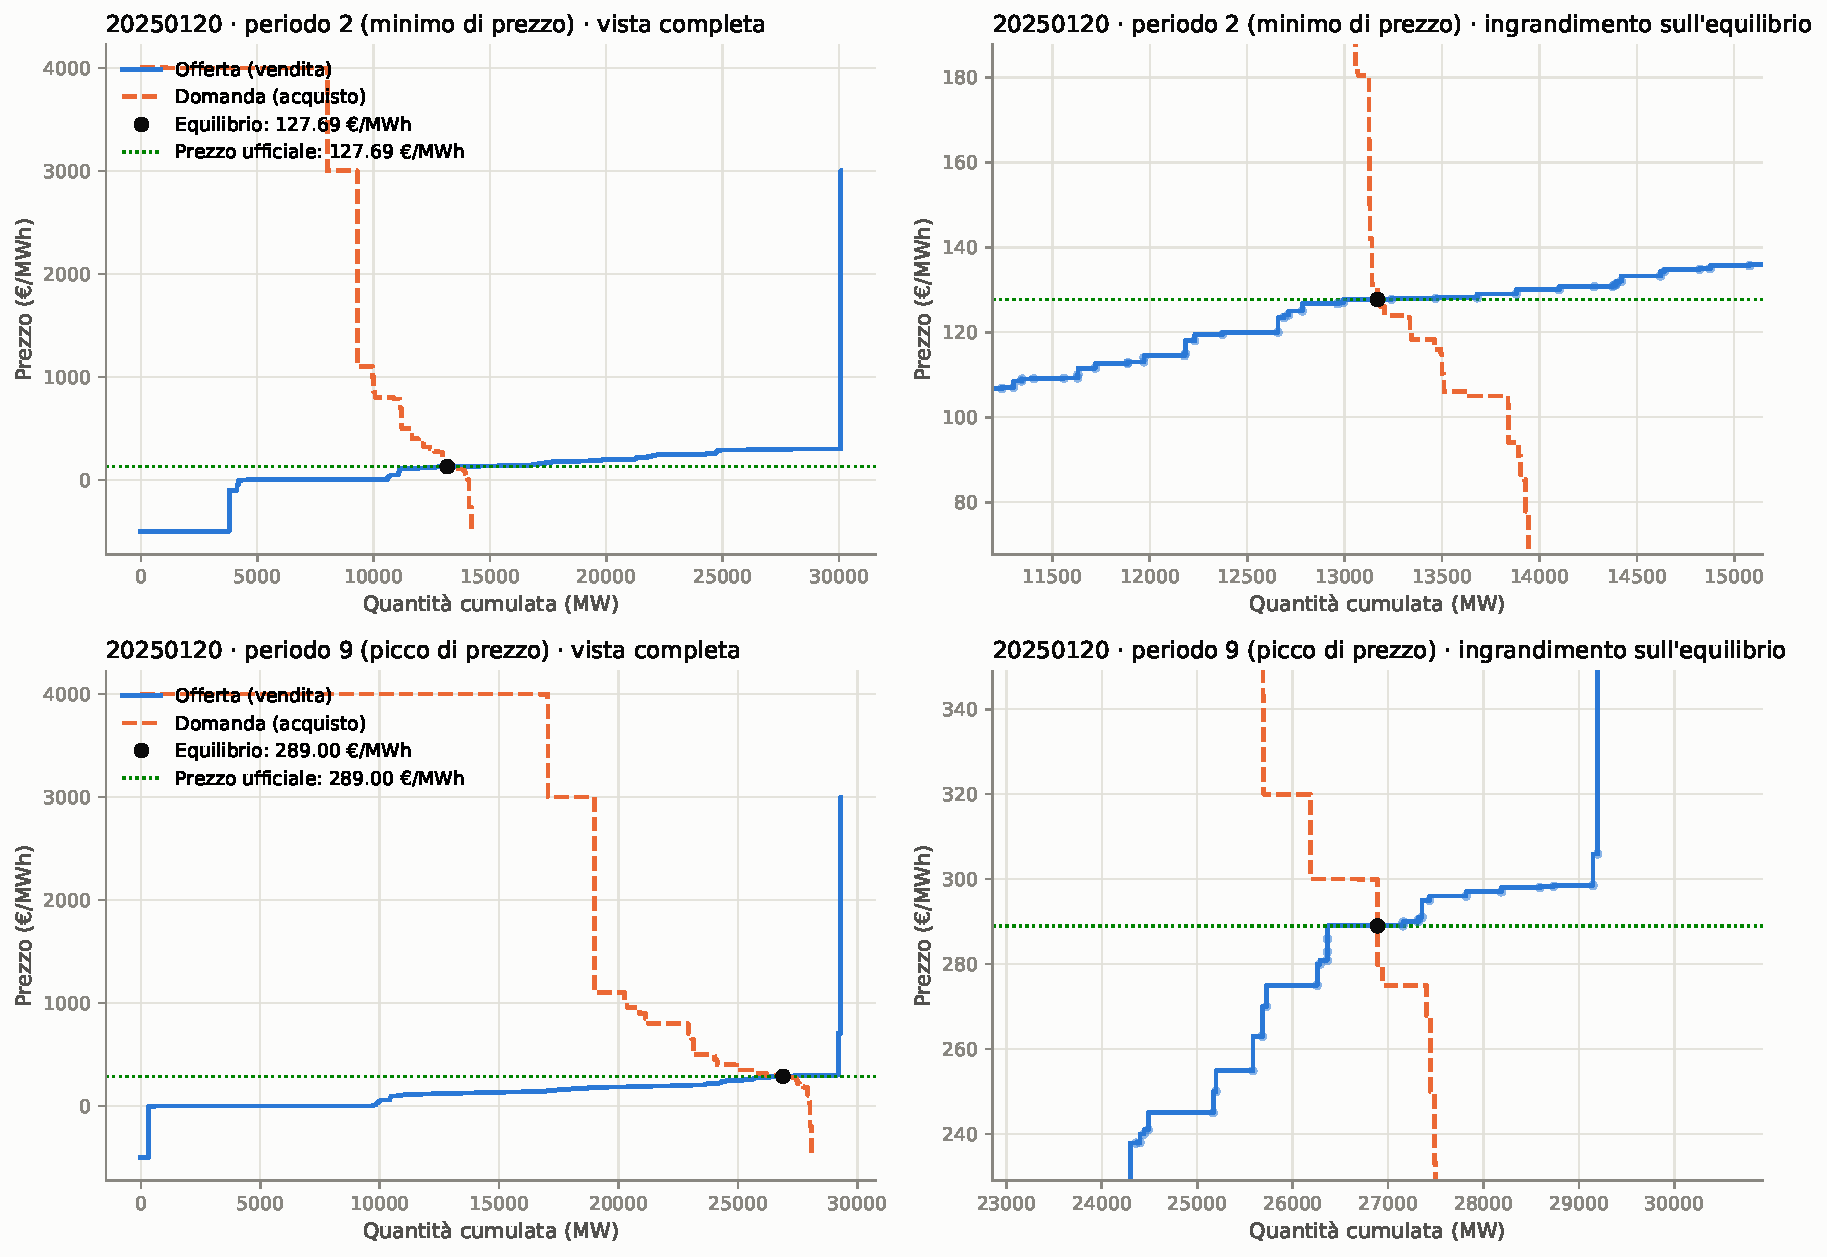
\includegraphics[width=\textwidth]{07_curve_20250120}
\caption{Curve aggregate di domanda e offerta ricostruite per l'ora di minimo (in alto) e
         quella di picco (in basso) del 20 gennaio 2025, in vista completa e ingrandite
         attorno all'equilibrio. I punti sulla curva di offerta sono i singoli gradini.}
\label{fig:curve}
\end{figure}

L'ispezione conferma tre cose. La pendenza attorno all'equilibrio poggia su \textbf{decine di
gradini}: nella finestra ingrandita ne cadono fra 39 e 62, ed entro $\pm 20$~\euromwh{} dal
prezzo di equilibrio si contano fra 42 e 72 offerte di vendita per 3.500-5.500~MW, la maggiore
delle quali vale circa un decimo del totale locale. Le offerte presentate ai \textbf{limiti di
prezzo} — il blocco a $-500$~\euromwh{} che occupa i primi migliaia di megawatt e la domanda
price taker a 4.000 — stanno agli estremi della curva e non toccano la regione di equilibrio.
Il prezzo ricostruito \textbf{cade dove atteso}: coincide con quello ufficiale al centesimo in
tre dei quattro periodi ispezionati, e nel quarto differisce di 1{,}50~\euromwh{} in un
periodo in cui la curva di offerta \`e visibilmente pi\`u piatta attorno all'incrocio.

Una caratteristica emerge con chiarezza dai grafici: la \textbf{curva di domanda \`e quasi
verticale} in corrispondenza dell'equilibrio, in tutti i periodi ispezionati. L'effetto
dell'accumulo passa quindi quasi interamente attraverso la curva di offerta, e ci\`o spiega
perch\'e sia la pendenza di quest'ultima a determinare la soglia.

\subsection{La curva di impatto marginale}
\label{sec:impatto}

Accanto al ricalcolo esatto dell'equilibrio, con cui si producono i risultati, \`e utile una
rappresentazione che renda leggibile in un colpo d'occhio quanto un periodo sia elastico: la
curva $\Delta p = f(\Delta q)$ della variazione di prezzo in funzione della quantit\`a aggiunta
o sottratta, con l'\textbf{origine centrata sul punto di clearing osservato} del periodo. La
tecnica \`e ripresa da \textcite{alonsoperez2026storage}, che la usano come proxy
dell'elasticit\`a del mercato spagnolo.

Si legge cos\`i: il ramo destro ($\Delta q > 0$) \`e l'accumulo che scarica, aggiunge offerta e
abbassa il prezzo; quello sinistro \`e l'accumulo che carica, aggiunge domanda e lo alza. I
tratti piatti sono i gradini larghi, dove l'accumulo passa inosservato; i salti sono i confini
fra un gradino e il successivo. L'asimmetria fra i due rami \`e la ragione per cui l'effetto
dell'accumulo non si riassume in un unico numero di elasticit\`a.

\begin{figure}[H]
\centering
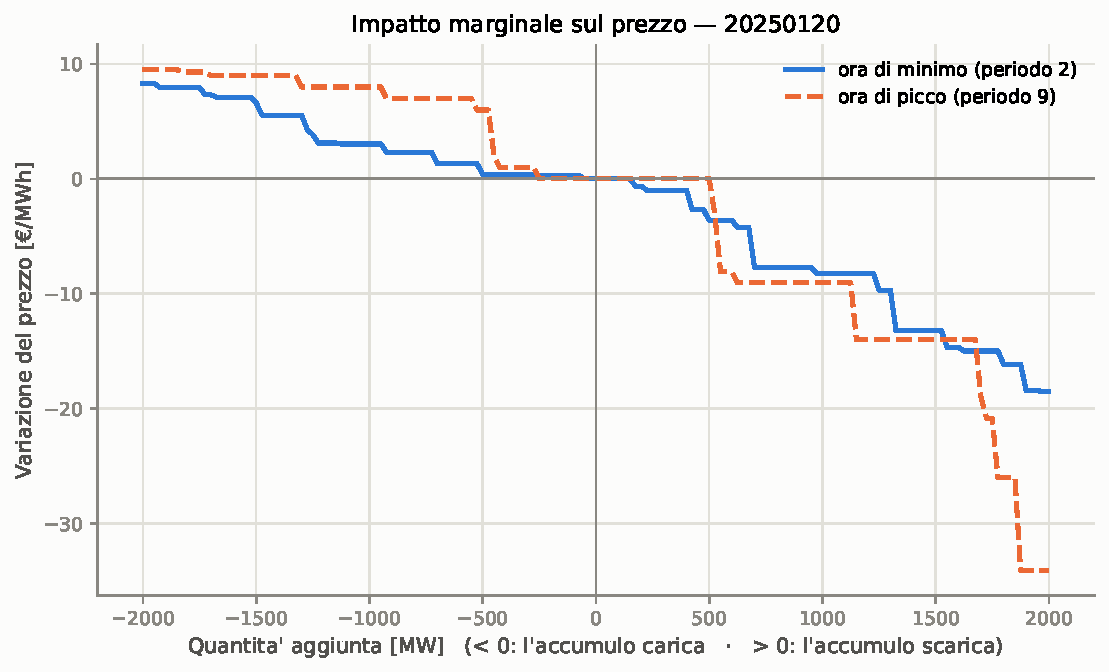
\includegraphics[width=\textwidth]{07_impatto_20250120}
\caption{Curva di impatto marginale dell'ora di minimo e dell'ora di picco del 20 gennaio
         2025. L'origine \`e il prezzo di equilibrio effettivamente ricostruito per quel
         periodo.}
\label{fig:impatto}
\end{figure}

La Figura~\ref{fig:impatto} rende visibile il meccanismo che governa l'intero risultato.
Attorno all'origine si estende un \textbf{pianoro} largo alcune centinaia di megawatt in cui il
prezzo non si muove affatto: l'equilibrio cade in mezzo a un gradino, e finch\'e l'accumulo non
lo esaurisce il prezzo marginale resta lo stesso. Superato il gradino la curva scende a
scalini, ciascuno dei quali \`e un'offerta che entra o esce dalla soluzione. \`E questa
struttura — non l'ampiezza del mercato — a determinare la soglia: ci\`o che conta \`e il
rapporto fra la taglia dell'accumulo e la larghezza dei gradini che attraversa.

La curva non \`e ottenuta ripetendo il clearing a ogni punto, ma invertendo la funzione di
eccesso di offerta. Aggiungere una quantit\`a $q$ di offerta price taker trasla $S(p)-D(p)$
verso l'alto di $q$ a ogni prezzo, da cui
\begin{equation}
p^{*}(q) \;=\; \min\left\{\, p \;:\; S(p) - D(p) \ge -q \,\right\},
\label{eq:impatto}
\end{equation}
che \`e esatta, non approssimata, e sfrutta la monotonia dell'eccesso di offerta gi\`a
richiamata nella Sezione~\ref{sec:mgp}.

Due limiti vanno dichiarati. La curva \`e una diagnostica \textbf{per periodo}, costruita a
curve fisse: non rivaluta le offerte a blocchi, che sono indivisibili e coprono pi\`u periodi,
quindi per capacit\`a elevate il prezzo che vi si legge pu\`o discostarsi da quello del
clearing di giornata. E l'asse in energia dipende dalla durata del periodo: su aste a quarto
d'ora un megawatt vale $0{,}25$~MWh, e le due scale coincidono soltanto sulle aste orarie.

\subsection{Il pavimento di discretezza}
\label{sec:pavimento}

Le curve ricostruite sono funzioni a gradini, e questo introduce un effetto che va corretto
prima di interpretare i risultati alle capacit\`a pi\`u piccole.

Con una griglia fitta nella parte bassa si osserva che fra 1 e 15~MW l'erosione cresce
\textbf{molto meno che proporzionalmente}: passa dallo 0{,}7\% all'1{,}3\% in mediana, cio\`e
raddoppia appena mentre la capacit\`a si moltiplica per quindici. Un effetto di mercato
dovrebbe invece scalare con la capacit\`a installata, e il valore a 1~MW dovrebbe essere
prossimo a zero.

L'esame periodo per periodo mostra la ragione: a 1~MW il prezzo si muove mediamente in due
periodi e mezzo sui tredici in cui l'accumulo opera, ma quando si muove \textbf{salta di un
gradino intero}, in media 1{,}4~\euromwh{}. Non \`e uno spostamento graduale: sono gli
equilibri che cadono esattamente sul bordo di un gradino e che pochi megawatt fanno scattare a
quello successivo.

Nel mercato reale il fenomeno non si presenta allo stesso modo, perch\'e l'offerta marginale
viene accettata parzialmente e l'incrocio cade all'interno del gradino. Si tratta quindi di un
\textbf{artefatto della ricostruzione}, non di un fenomeno da misurare.

Il pavimento viene misurato alla capacit\`a pi\`u piccola della griglia — dove per costruzione
non pu\`o esserci effetto di mercato — e sottratto giorno per giorno. Vale lo 0{,}7\% in
mediana e il 2{,}8\% al 90\textsuperscript{o} percentile. La correzione sposta la soglia in
modo sistematico, e in misura tanto maggiore quanto pi\`u basso \`e il livello di erosione
scelto: a un livello del 20\% la sposta del 21\%, al 10\% del 75\%, al 5\% del 117\%. Ne segue
che una soglia fissata al 5\% \`e la \textbf{meno affidabile}, perch\'e il pavimento vale pi\`u
della met\`a della soglia stessa.

\subsection{Dal campione alla soglia: il bootstrap}
\label{sec:bootstrap}

La soglia $K^*$ si stima ricampionando i giorni con reimmissione. Per ciascun
ricampionamento si calcola, a ogni capacit\`a della griglia, il quantile prudenziale
dell'erosione fra i giorni estratti; si ottiene cos\`i una curva che lega il quantile alla
capacit\`a, crescente perch\'e pi\`u accumulo erode di pi\`u; e si individua per interpolazione
la capacit\`a alla quale quella curva attraversa il livello di erosione dichiarato. La
distribuzione delle $K^*$ cos\`i ottenute fornisce l'intervallo di confidenza.

Due scelte vanno dichiarate perch\'e non sono stimate dai dati. Il \textbf{livello di
erosione} che definisce il passaggio a price maker \`e convenzionale: si adotta il 10\%, e la
sensibilit\`a a questa scelta \`e riportata nel Capitolo~\ref{cap:valutazione}. Il
\textbf{quantile} \`e l'80\textsuperscript{o} o il 90\textsuperscript{o} percentile, e non uno
pi\`u estremo: con qualche centinaio di giorni un quantile al 95\textsuperscript{o} o al
99\textsuperscript{o} percentile poggerebbe su pochissime osservazioni e la sua stima sarebbe
instabile proprio nella parte che determina il risultato.

\subsection{Le giornate a basso differenziale}
\label{sec:basso-spread}

Quando il differenziale di prezzo giornaliero \`e piccolo, $\pi_{PT}$ tende a zero e il
rapporto~\eqref{eq:erosione} diventa privo di significato o esplode. Scartare quelle giornate
sarebbe per\`o metodologicamente pericoloso: sono le giornate ad alta produzione rinnovabile
e prezzi compressi, cio\`e proprio quelle destinate a diventare pi\`u frequenti, e escluderle
introdurrebbe un \textbf{bias sistematico} nella direzione opposta a quella dell'evoluzione
del sistema.

La scelta \`e quindi di mantenerle nel campione e di riportare, accanto all'erosione
relativa, anche quella in \textbf{valore assoluto} (euro al giorno), che resta interpretabile
a qualunque livello di differenziale. Il rapporto viene semplicemente omesso dove il profitto
di riferimento \`e trascurabile, e il numero di casi in cui ci\`o accade \`e riportato con i
risultati.

\section{La fase previsiva e la struttura del suo errore}
\label{sec:previsione}

La fase 1 dell'impianto a due fasi (Sezione~\ref{sec:due-fasi}) produce, per ogni giorno del
campione, la previsione delle ventiquattro ore successive formulata con la sola informazione
disponibile alla chiusura del mercato. Questa sezione ne descrive la specifica e, soprattutto,
\textbf{caratterizza l'errore che ne risulta}: non per misurare l'accuratezza del modello, che
non \`e l'oggetto della tesi, ma perch\'e \`e la struttura di quell'errore a propagarsi al
piano dell'accumulo e al risultato economico.

\subsection{L'orizzonte, e perch\'e \`e esattamente ventiquattro}

Il \ac{MGP} del giorno $D$ chiude a mezzogiorno di $D-1$, ma gli esiti di $D-1$ sono stati
pubblicati il giorno prima: al momento della decisione l'operatore conosce \textbf{tutte} le
ventiquattro ore di $D-1$ e nessuna di $D$. L'origine della previsione \`e quindi la fine di
$D-1$ e l'orizzonte $h = 1, \dots, 24$. Nessuna informazione dal futuro entra nel piano, e non
serve troncare la giornata a met\`a.

Si prevedono i prezzi zonali \textbf{ufficiali} pubblicati dal \ac{GME}, non quelli
ricostruiti dal modello di clearing. \`E quello che osserva un operatore reale, e prevedere la
propria ricostruzione significherebbe prevedere anche il proprio errore di ricostruzione, che
non \`e un fenomeno di mercato. La scelta non intacca l'erosione, perch\'e la fase 2 continua
a valorizzare sui prezzi ricostruiti con e senza accumulo: l'errore di ricostruzione entra
identico nei due termini e si semplifica.

\subsection{La specifica}
\label{sec:specifica}

Si adotta un modello \ac{SARIMAX} nella formulazione classica di
\textcite{box2015timeseries}, e non un metodo di apprendimento automatico. La ragione discende
dall'oggetto: poich\'e interessa la \emph{struttura} dell'errore e non la sua sola dimensione,
serve un modello con una teoria dell'errore esplicita --- intervalli di previsione derivati,
residui analizzabili --- e non soltanto misurabile a posteriori. \textcite{weron2014previsione}
documenta del resto che i modelli di questa famiglia restano il termine di confronto
obbligato nella previsione dei prezzi elettrici, qualunque sia il metodo che li affianca.

La specifica adottata \`e
\[
  \text{SARIMAX}(2,1,1)\times(0,1,1)_{24}
\]
con regressori esogeni deterministici.

\paragraph{La parte stagionale non \`e una scelta ma una lettura.} Sulla serie oraria della
zona NORD, la \ac{ACF} della sola differenza prima ai multipli di ventiquattro vale
$+0{,}62$, $+0{,}57$, $+0{,}53$, $+0{,}53$, $+0{,}52$: \textbf{non decade}, cio\`e resta una
stagionalit\`a non rimossa. Aggiungendo la differenza stagionale i medesimi valori diventano
$-0{,}43$, $-0{,}01$, $-0{,}05$, $+0{,}00$, $-0{,}06$: una \textbf{sola punta negativa a
ritardo ventiquattro che poi taglia netto}, con \ac{PACF} pari a $-0{,}429$. \`E la firma di
una media mobile stagionale di ordine uno, da cui $D = 1$, $P = 0$, $Q = 1$, $s = 24$.

\paragraph{La stagionalit\`a settimanale entra come regressore, non come seconda
stagionalit\`a.} Un modello SARIMA ne ammette una sola, e differenziare a ritardo
centosessantotto costerebbe una settimana di osservazioni iniziali. Si usano invece due coppie
di termini di Fourier a periodo $168$ e tre indicatrici, per sabato, domenica e festivi
italiani. La scelta \`e sostenuta dai dati: tolto il profilo orario, il giorno della settimana
spiega il \SI{5,2}{\percent} della varianza residua, con un'escursione di
15,8~\euromwh{}. Merita qualche regressore, non una struttura stagionale.

\paragraph{Nessuna trasformazione logaritmica.} Il minimo osservato nel biennio vale
0,10~\euromwh{} e sul \ac{MGP} i prezzi negativi sono ammessi fino a
$-500$~\euromwh{}: il logaritmo sarebbe fragile per costruzione.

\paragraph{Ordine congelato.} Gli ordini non stagionali sono stati scelti confrontando per
\ac{AIC} quattro candidati dichiarati in anticipo, \emph{una volta sola} sull'anno di
addestramento, e poi \textbf{congelati} per tutto il periodo di valutazione. Sono cio\`e un
dato dichiarato del lavoro, non un iperparametro riottimizzato a ogni passo.

\paragraph{Protocollo a origine mobile.} Per ogni giorno del campione si producono
ventiquattro passi con origine alla fine del giorno precedente. I coefficienti si ristimano
una volta al mese, non ogni giorno: sia perch\'e trecentosessantasei stime complete
costerebbero giorni di calcolo per un guadagno previsivo trascurabile, sia perch\'e nessun
operatore ricalibra un modello ogni notte. Fra una ristima e l'altra il filtro assorbe il
giorno appena osservato aggiornando lo \emph{stato} senza toccare i \emph{coefficienti}.

\subsection{La struttura dell'errore, in sei dimensioni}
\label{sec:errore}

Sia $e(g,h)$ l'errore del giorno $g$ all'ora $h$, definito come prezzo reale meno prezzo
previsto: positivo dove il modello ha sottostimato. Sull'anno di valutazione l'errore vale
14,75~\euromwh{} di \ac{RMSE} e 10,54 di \ac{MAE}. Sono numeri che da soli
non dicono nulla di utile: quello che conta \`e come si distribuiscono.

\paragraph{1. Per ora del giorno.} L'errore non \`e omogeneo: varia di \textbf{2,4 volte} fra
l'ora migliore e la peggiore, da 8,22~\euromwh{} a mezzanotte a 19,97 alle
quattordici (Figura~\ref{fig:errore-orario}). Le ore notturne, piatte, si prevedono bene; il
pomeriggio male.

Il fattore che lo spiega non \`e il livello del prezzo ma la sua \textbf{variabilit\`a}: la
correlazione fra l'errore orario e la deviazione standard del prezzo in quell'ora vale
$+0{,}931$, contro $+0{,}185$ con il livello medio. Il picco serale, che \`e l'ora di prezzo
pi\`u alto dell'anno, si prevede \emph{meglio} del ventre pomeridiano, perch\'e \`e alto ma
regolare, mentre il pomeriggio \`e mediamente basso ma erratico, dipendendo dal fotovoltaico.

Il rilievo per l'arbitraggio \`e diretto: la batteria colloca spesso la carica proprio nel
ventre pomeridiano, che \`e l'ora peggio prevista dell'intera giornata.

\paragraph{2. Distorsione contro dispersione.} Il modello \`e \textbf{non distorto}: media
dell'errore $0{,}015$~\euromwh{}, con un test $t$ sulla media nulla che d\`a $p = 0{,}93$. Il
massimo bias per ora del giorno vale $0{,}29$~\euromwh{} contro una dispersione di
$14{,}75$. Tutto l'errore \`e dunque dispersione, non distorsione sistematica: non esiste una
correzione da applicare, si pu\`o solo convivere con la varianza.

\paragraph{3. Code e forma.} La distribuzione \`e simmetrica (asimmetria $-0{,}0002$) ma
decisamente \textbf{leptocurtica}: curtosi in eccesso $+3{,}97$
(Figura~\ref{fig:errore-forma}). Gli eventi oltre tre deviazioni standard sono \textbf{6,2
volte} pi\`u frequenti dell'attesa gaussiana, quelli oltre quattro \textbf{101 volte}.
L'\SI{1}{\percent} peggiore delle ore porta il \SI{19,0}{\percent} della somma dei quadrati,
il \SI{5}{\percent} peggiore il \SI{45,4}{\percent}.

Questo si lega alla redditivit\`a in modo diretto. L'errore quadratico medio giornaliero
correla con il differenziale del giorno a $r = +0{,}600$ e con la volatilit\`a a $r =
+0{,}638$, mentre con il livello medio dei prezzi non correla affatto ($r = +0{,}045$, non
significativo). L'errore \`e cio\`e massimo proprio nelle giornate in cui l'arbitraggio vale
di pi\`u. Il modello inoltre \textbf{contrae il differenziale} verso la sua media: prevede
valori compresi fra 40 e 80~\euromwh{} quando il reale spazia da 20 a
158, e lo sottostima nel \SI{65}{\percent} delle giornate
(Figura~\ref{fig:errore-spread}).

\paragraph{4. Autocorrelazione.} L'\ac{ACF} dei residui vale $+0{,}849$ a ritardo uno,
$+0{,}670$ a due, $+0{,}518$ a tre; la \ac{PACF} vale $+0{,}849$ a uno, $-0{,}184$ a due e
poi si annulla. Il test di Ljung-Box rifiuta l'ipotesi di residui incorrelati con $p$
inferiore a $10^{-4}$ a tutti i ritardi esaminati. Il trattamento di questo limite \`e nella
Sezione~\ref{sec:limiti-previsione}.

La memoria vive per\`o \textbf{dentro} la giornata e non fra giornate: l'\ac{ACF} dell'errore
medio giornaliero vale $+0{,}034$ a ritardo uno, dentro la banda di non significativit\`a. Una
giornata difficile non ne annuncia un'altra. \`E il verso peggiore per il piano: un errore
coerente per l'intera giornata sbaglia l'\emph{ordinamento} delle ore, mentre errori
indipendenti si compenserebbero fra loro.

\paragraph{5. Eteroschedasticit\`a.} Rispetto al \emph{livello} del prezzo previsto l'errore
segue un andamento \textbf{a U}: \ac{RMSE} pari a $22{,}01$ nel decile pi\`u basso,
$10{,}96$ nei centrali, $20{,}63$ nel pi\`u alto. Una correlazione di rango non lo
rivelerebbe --- vale $+0{,}001$, non significativa --- perch\'e cerca monotonia dove la
relazione non \`e monotona.

Rispetto alla \textbf{volatilit\`a della giornata} la relazione \`e invece monotona e forte:
l'errore medio passa da $9{,}93$ nel quintile pi\`u tranquillo a $20{,}45$ nel pi\`u agitato.
\`E l'anello che lega l'errore di previsione al regime di mercato, e va nella direzione
sfavorevole: i regimi volatili sono quelli in cui l'accumulo guadagna.

I decili si costruiscono sul prezzo \emph{previsto} e non su quello realizzato. Raggruppare
per il realizzato sarebbe contaminato per costruzione, perch\'e nel gruppo dei prezzi alti
finirebbero per definizione le ore in cui il prezzo \`e stato pi\`u alto del previsto: si
misurerebbe una regressione verso la media, non l'eteroschedasticit\`a.

\paragraph{6. Calibrazione degli intervalli.} La copertura empirica degli intervalli di
previsione, confrontata con quella nominale, decresce in modo monotono e cambia segno:
\SI{64,7}{\percent} contro un nominale del \SI{50}{\percent}, 88,2 contro
80, 93,6 contro 90, 96,0 contro 95,
98,1 contro 99 (Figura~\ref{fig:calibrazione}).

\`E la firma esatta di intervalli gaussiani costruiti su un errore leptocurtico: troppo larghi
al centro, troppo stretti nelle code. Il difetto non \`e di \emph{ampiezza} ma di
\emph{forma}, ed \`e la stessa cosa vista al punto 3, letta dal lato dell'incertezza
dichiarata. La miscalibrazione \`e inoltre strutturata per ora: la copertura al
\SI{90}{\percent} vale 97--\SI{99}{\percent} nelle ore notturne e scende a
86,9--\SI{88,8}{\percent} fra le tredici e le quindici, cio\`e il modello \`e pi\`u
sicuro di quanto dovrebbe proprio nelle ore che contano per l'arbitraggio.

\subsection{Due limiti dichiarati}
\label{sec:limiti-previsione}

\paragraph{I residui non sono bianchi, e va detto per primo.} L'autocorrelazione dei residui
vale $+0{,}849$ a ritardo uno e il test di Ljung-Box rifiuta con $p$ inferiore a $10^{-4}$.
Resta quindi \textbf{struttura non catturata}: il modello \`e migliorabile in senso
statistico, e sarebbe scorretto presentarlo come adeguato.

Questo per\`o \textbf{non intacca il risultato economico}, e la ragione non \`e una
minimizzazione ma una conseguenza di quanto stabilito nella Sezione~\ref{sec:ordinale}.
L'autocorrelazione residua riguarda il \emph{livello} dei prezzi --- \`e su quello che il
modello lascia segnale non sfruttato --- mentre il valore dell'arbitraggio dipende
dall'\emph{ordinamento} delle ore. Un modello con residui pi\`u bianchi produrrebbe previsioni
di livello migliori, ma ridurrebbe il costo del \SI{10,4}{\percent} solo nella misura in cui
migliorasse specificamente la classifica delle ore, che \`e una propriet\`a diversa e che
nessuno dei criteri usuali di adattamento misura.

Ne segue anche un'indicazione per chi volesse proseguire: raffinare il modello sul criterio
d'informazione o sulla bianchezza dei residui \`e la strada meno promettente. Converrebbe
piuttosto valutarlo direttamente sulla correlazione di rango giornaliera, che \`e la
statistica che determina il piano.

\paragraph{Ora del giorno e orizzonte non sono separabili.} L'origine della previsione \`e
sempre la fine di $D-1$, quindi l'orizzonte $h$ corrisponde sempre e solo all'ora $h-1$ del
giorno $D$: le due variabili sono \textbf{collineari per costruzione} e nessuna analisi su
questi dati pu\`o attribuire all'una o all'altro lo schema osservato. Non \`e un difetto del
disegno statistico ma della struttura del mercato, che ammette una sola sessione al giorno.

Si pu\`o per\`o escludere che si tratti di un puro effetto di orizzonte. Un errore crescente
con la distanza temporale sarebbe monotono, e lo schema non lo \`e: vale
8,22~\euromwh{} alla prima ora, sale a 19,97 alla quindicesima e ridiscende
a 10,65 alla ventiquattresima. Il coefficiente di correlazione fra errore orario e
variabilit\`a del prezzo in quell'ora vale $+0{,}931$, contro $+0{,}185$ con il livello: il
fattore dominante \`e l'ora, non la distanza.

\begin{figure}[H]
\centering
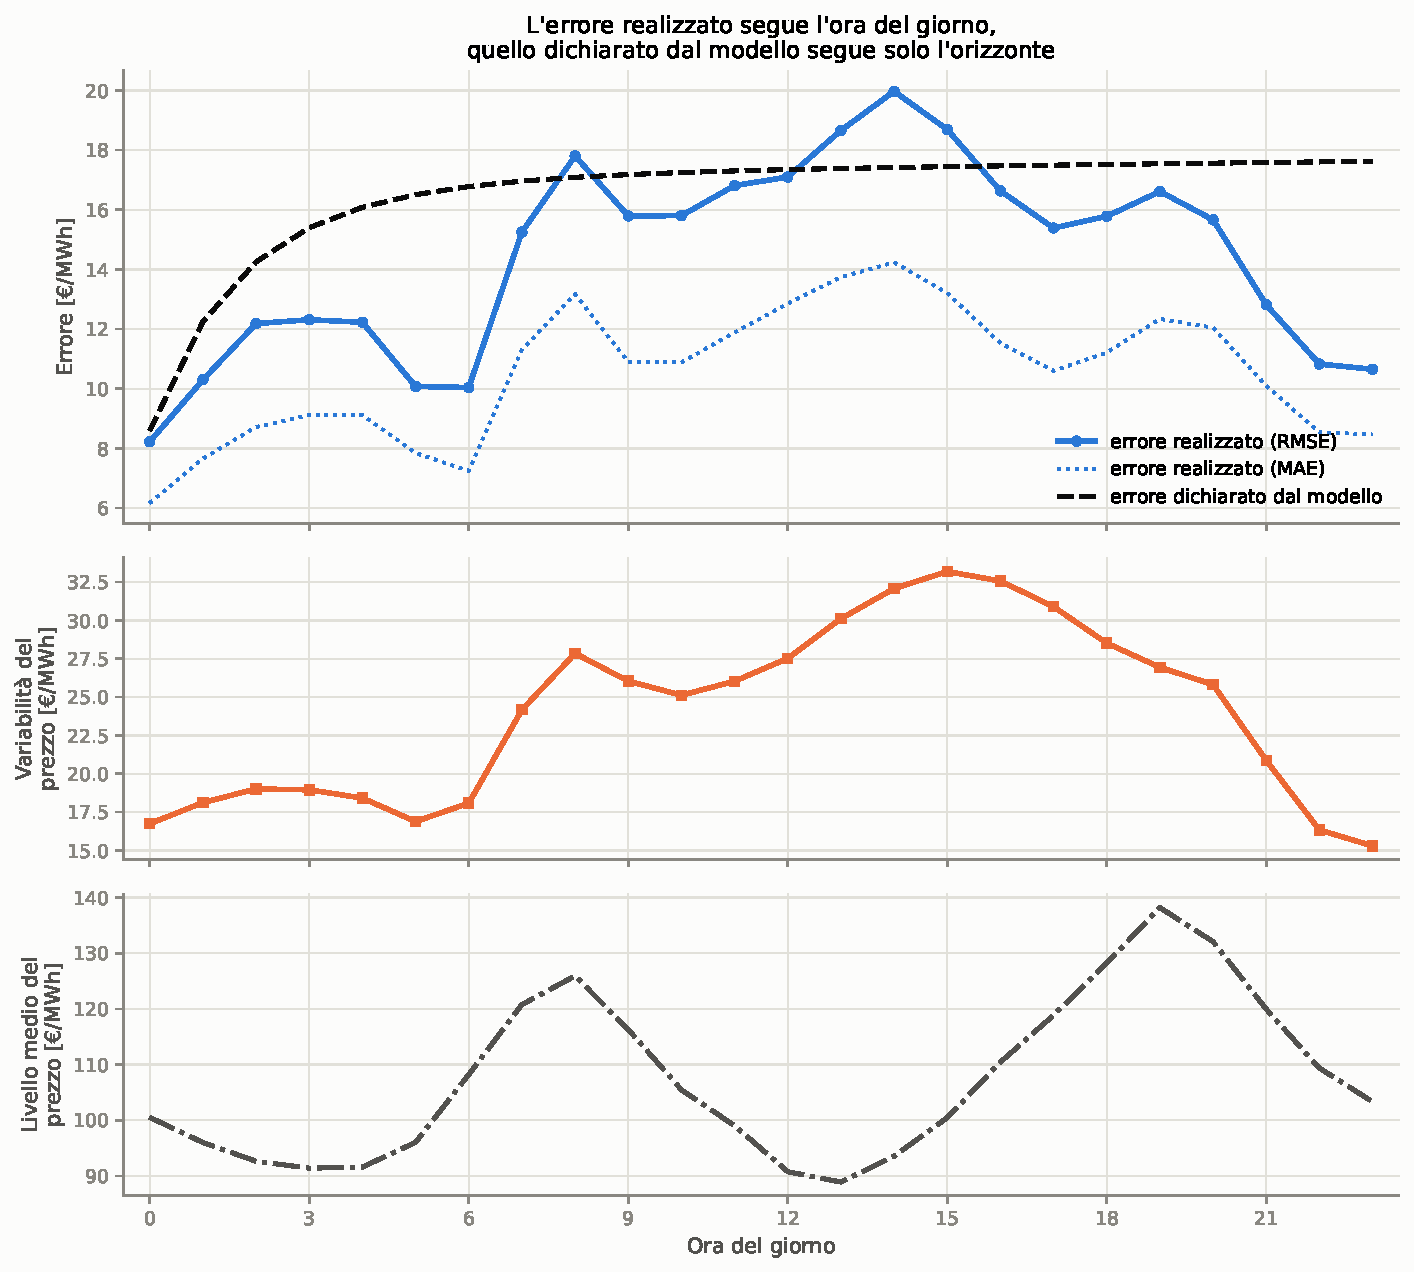
\includegraphics[width=0.92\textwidth]{15_errore_orario}
\caption{Errore di previsione per ora del giorno. In alto l'errore realizzato, in due
metriche, contro quello \emph{dichiarato} dal modello: il secondo cresce in modo monotono con
l'orizzonte, come impone la teoria, mentre il primo segue l'ora del giorno. Al centro la
variabilit\`a del prezzo in ciascuna ora, che ha la stessa forma dell'errore ($r = +0{,}931$);
in basso il livello medio, che ne ha una diversa ($r = +0{,}185$).}
\label{fig:errore-orario}
\end{figure}

\begin{figure}[H]
\centering
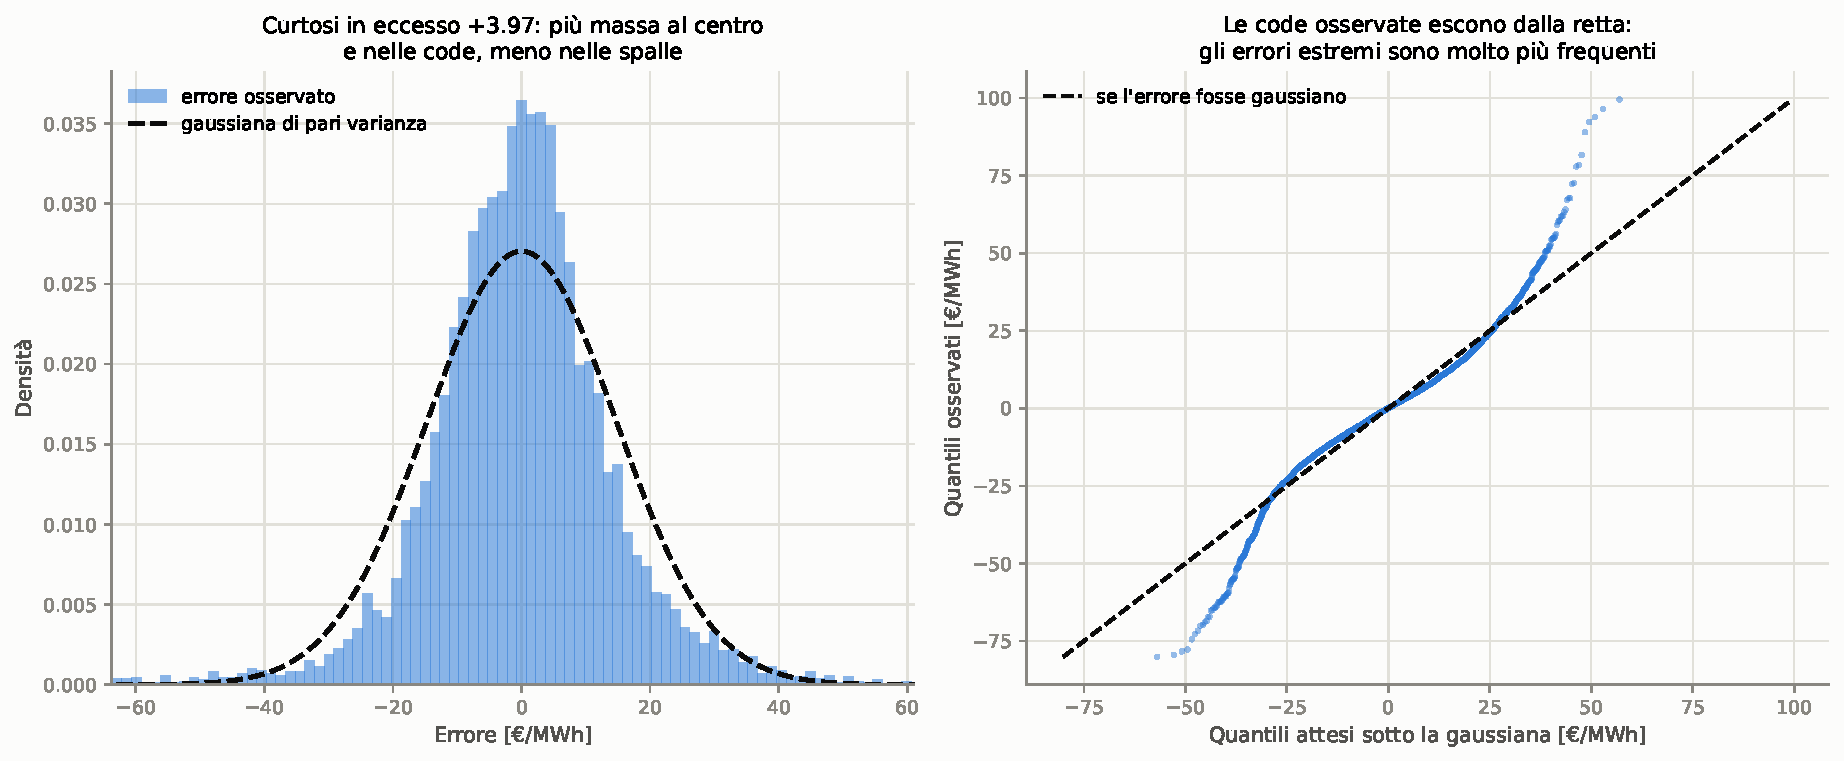
\includegraphics[width=\textwidth]{15_errore_forma}
\caption{Forma della distribuzione dell'errore. L'istogramma da solo ingannerebbe, perch\'e le
code sono rare proprio dove contano; il diagramma quantile-quantile le rende leggibili come
scostamento dalla bisettrice.}
\label{fig:errore-forma}
\end{figure}

\begin{figure}[H]
\centering
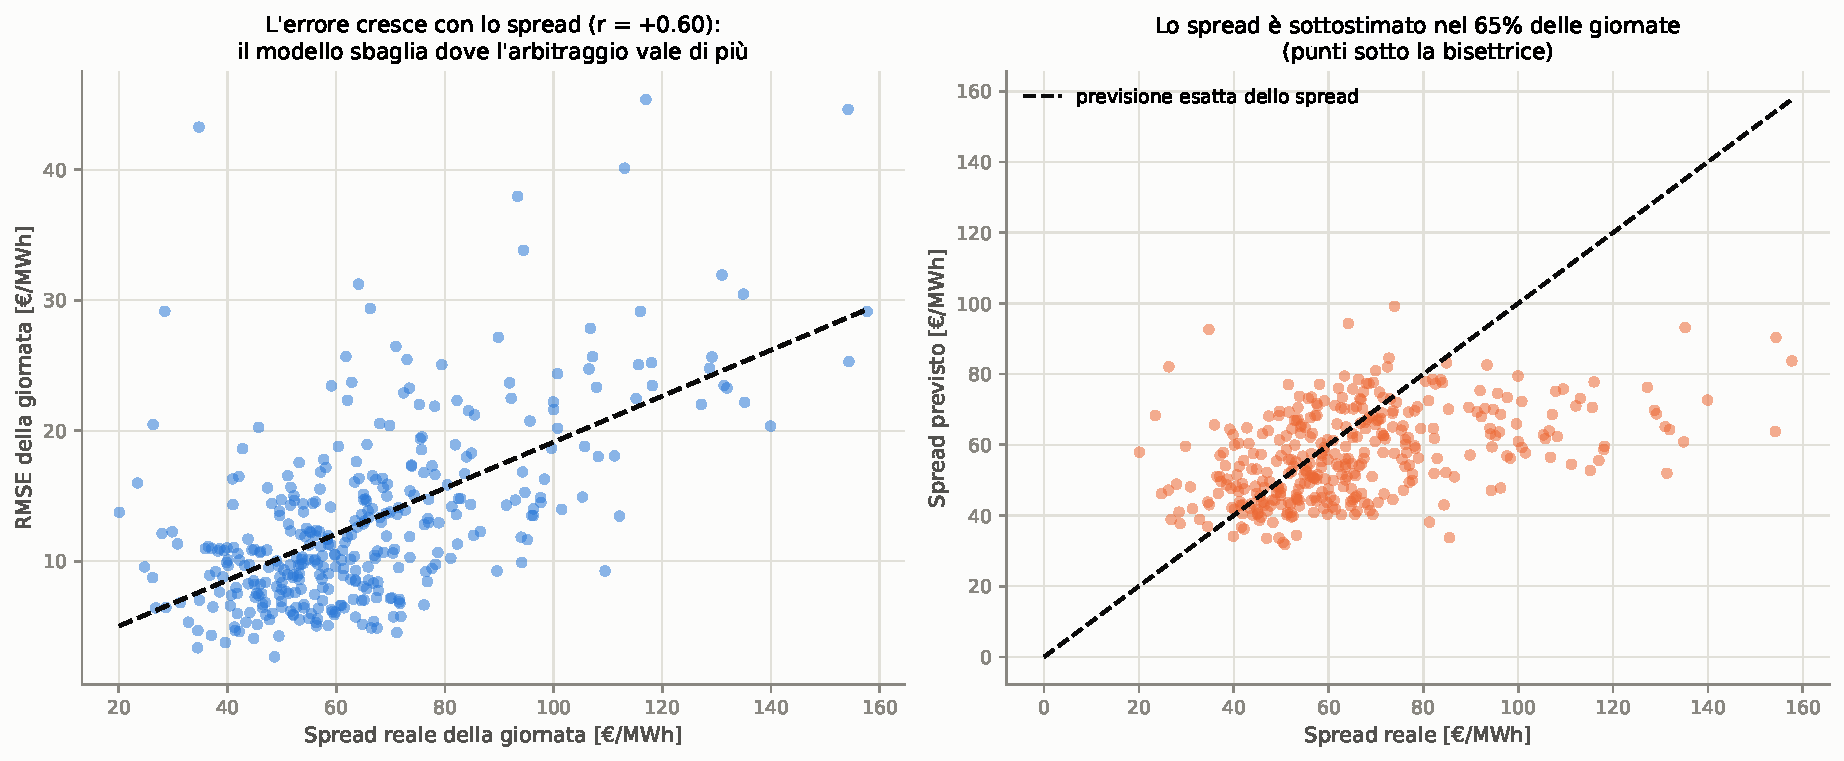
\includegraphics[width=\textwidth]{15_errore_spread}
\caption{A sinistra, l'errore giornaliero cresce con il differenziale della giornata: il
modello sbaglia di pi\`u dove l'arbitraggio vale di pi\`u. A destra, il differenziale
previsto resta confinato in una fascia stretta mentre quello reale spazia molto di pi\`u:
il modello lo contrae verso la sua media.}
\label{fig:errore-spread}
\end{figure}

\begin{figure}[H]
\centering
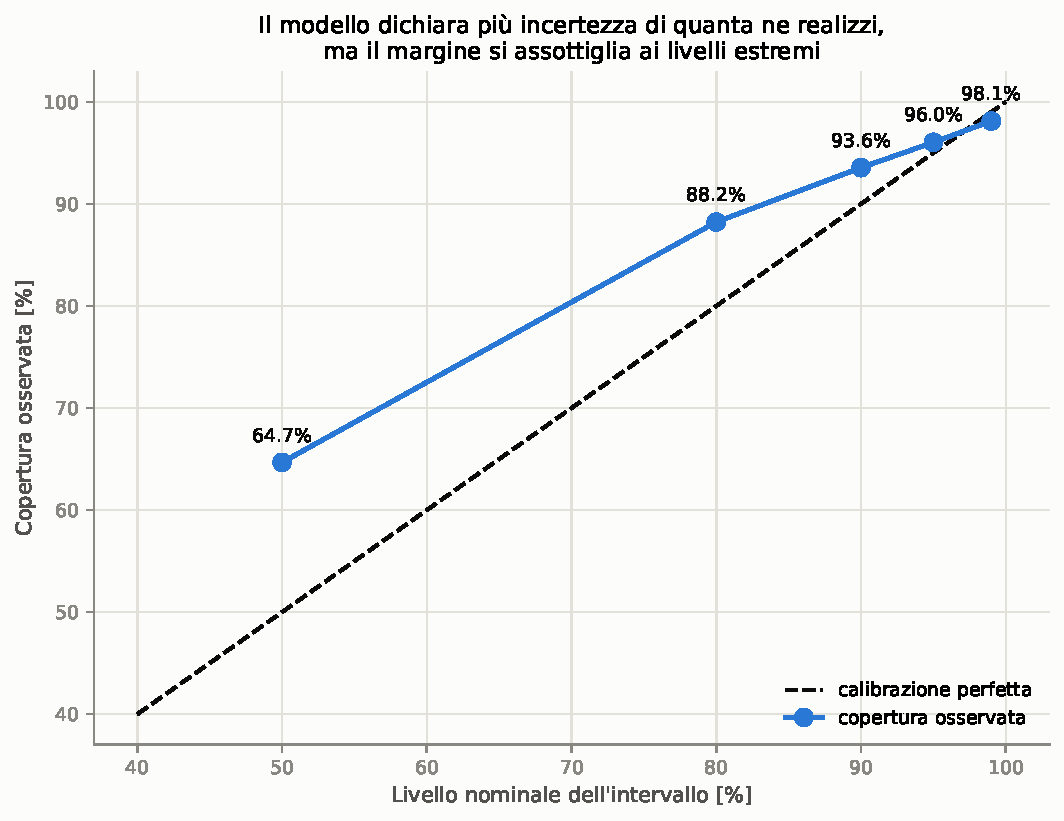
\includegraphics[width=0.78\textwidth]{15_calibrazione}
\caption{Copertura empirica contro copertura nominale degli intervalli di previsione. Lo
scarto decresce in modo monotono e cambia segno: \`e la firma di intervalli gaussiani su un
errore a code spesse.}
\label{fig:calibrazione}
\end{figure}

\section{La soglia $K^*$}
\label{sec:soglia-definitiva}

La soglia si stima sulla griglia definitiva a 132 capacit\`a, con l'erosione al netto del
pavimento di discretezza (Sezione~\ref{sec:pavimento}) e le giornate a piano vuoto contate a
erosione nulla. Si riportano \textbf{due varianti}: piano da previsione perfetta, che \`e il
riferimento, e piano da previsione (Sezione~\ref{sec:due-varianti}).

\subsection{La verifica preliminare di monotonia}

La regola con cui si individua $K^*$ prende il \emph{primo} superamento della soglia da parte
della curva quantile, il che presuppone che la curva sia crescente. Con una griglia fitta un
sobbalzo locale del quantile dentro un ricampionamento potrebbe farla scattare in anticipo e
abbassare la stima: la presunzione va quindi verificata prima di usare il risultato, non dopo.

Su mille ricampionamenti e per tutte e quattro le combinazioni di variante e soglia, la quota
di ricampionamenti con \textbf{pi\`u di un attraversamento \`e nulla}, il calo massimo della
curva vale $-0{,}01$ punti percentuali in mediana, e lo scarto fra ultimo e primo
attraversamento \`e \textbf{esattamente zero}, sia in media sia al massimo. La regola del
primo attraversamento resta quindi valida e non serve alcuna correzione.

\subsection{Il risultato}

\begin{table}[H]
\centering
\caption{Soglia $K^*$ al 90\textsuperscript{o} percentile dell'erosione netta, con intervallo
di confidenza al \SI{90}{\percent} da mille ricampionamenti dei giorni.}
\label{tab:soglia}
\begin{tabular}{@{}llrr@{}}
\toprule
\textbf{Piano} & \textbf{Soglia} & \textbf{$K^*$ (MW)} & \textbf{IC \SI{90}{\percent}} \\
\midrule
previsione perfetta  & \SI{10}{\percent} & 75,9  & 70,5 -- 81,7 \\
previsione perfetta  & \SI{20}{\percent} & 173,1 & 157,5 -- 189,0 \\
da previsione        & \SI{10}{\percent} & 50,1  & 43,3 -- 57,5 \\
da previsione        & \SI{20}{\percent} & 129,3 & 108,0 -- 142,9 \\
\bottomrule
\end{tabular}
\end{table}

\textbf{La differenza fra le due varianti \`e il risultato}: la soglia scende del
\SI{34,0}{\percent} al livello del \SI{10}{\percent} e del \SI{25,3}{\percent} al
\SI{20}{\percent}. Gli intervalli di confidenza delle due varianti non si sovrappongono a
nessuna delle due soglie, quindi la differenza non \`e un artefatto campionario.

Una flotta che pianifica su previsioni realistiche diventa price maker \textbf{prima}. Lo
stesso errore che le costa il \SI{10,4}{\percent} di profitto la fa anche operare in modo meno
mirato, quindi con pi\`u effetto sul prezzo a parit\`a di capacit\`a installata --- e lo
conferma anche l'erosione in valore assoluto, non solo il rapporto.

\paragraph{Quanto pesa il pavimento.} Sulla stessa griglia, ma senza sottrarre il pavimento di
discretezza, la soglia della variante realistica risulterebbe di \SI{33,7}{MW} invece di
50,1. La correzione del pavimento non \`e quindi un raffinamento marginale: senza di
essa la soglia sarebbe sottostimata di un terzo.

\paragraph{Una sensibilit\`a da dichiarare.} Il pavimento \`e mal definito nelle giornate in
cui il profitto di riferimento \`e quasi nullo, dove il rapporto \`e dominato dal rumore: due
giornate su trecentosessantasei superano il \SI{25}{\percent} di pavimento, e in una di esse
il profitto a \SI{1}{MW} vale meno di cinque euro. Escludendo le giornate a pavimento anomalo
il divario fra le due varianti resta compreso fra il 26 e il \SI{34}{\percent}, quindi
il risultato qualitativo \`e robusto, ma il valore puntuale ne dipende. Si adotta la stima sul
campione completo, coerentemente con la scelta di non scartare le giornate a basso
differenziale (Sezione~\ref{sec:basso-spread}), dichiarando la sensibilit\`a.

\begin{figure}[H]
\centering
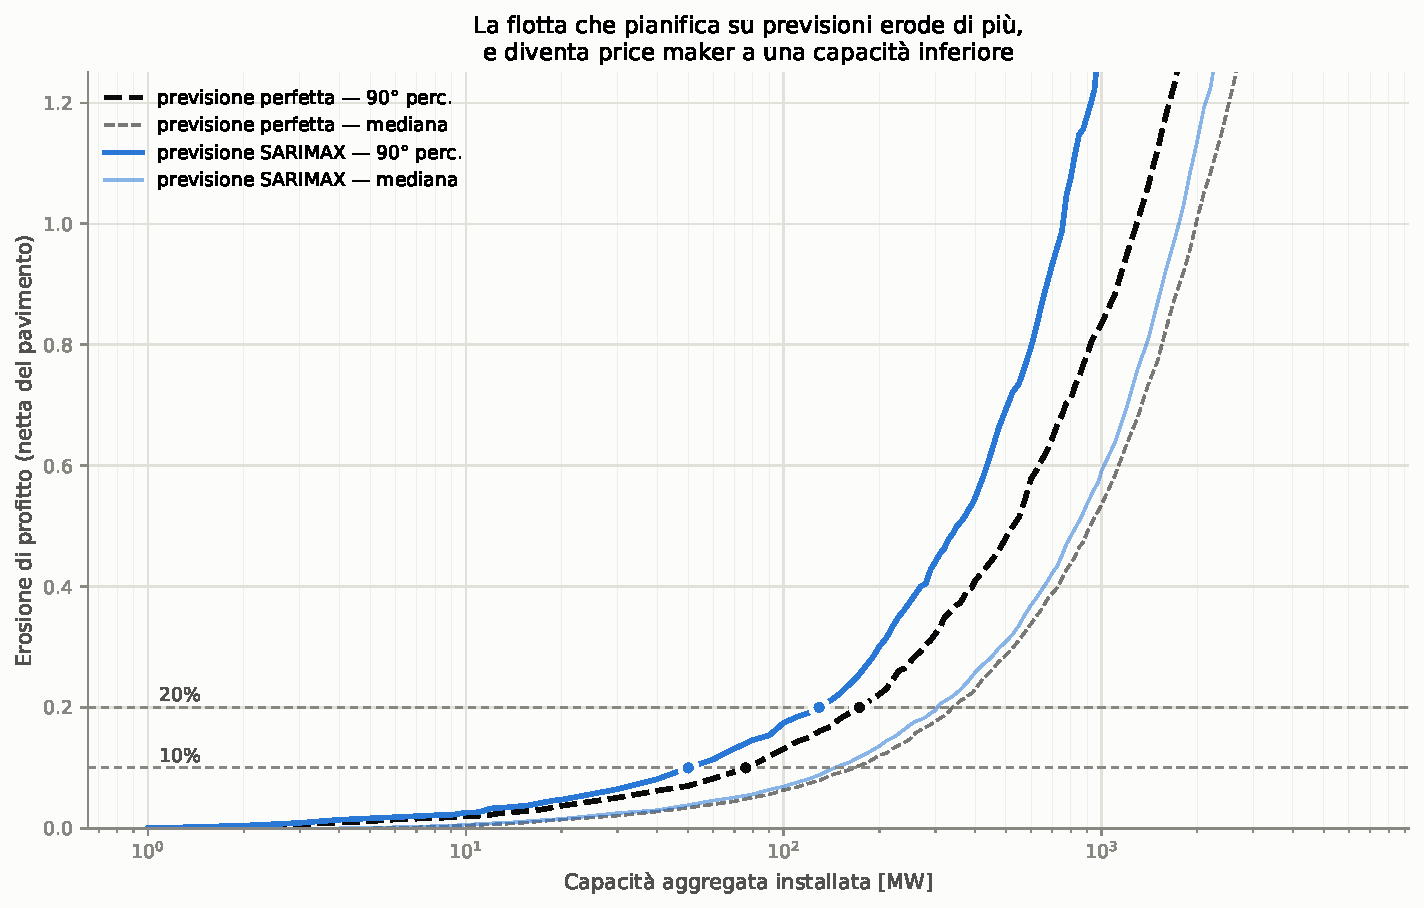
\includegraphics[width=0.95\textwidth]{17_curva_erosione}
\caption{Curva erosione-capacit\`a nelle due varianti di piano, mediana e
90\textsuperscript{o} percentile, su scala logaritmica delle capacit\`a. La curva della
variante realistica sta sopra quella della previsione perfetta a ogni capacit\`a: i punti
segnano i quattro $K^*$ della Tabella~\ref{tab:soglia}.}
\label{fig:curva-erosione}
\end{figure}

\subsection{La propagazione dell'errore al piano}
\label{sec:propagazione}

Il confronto fra le due varianti permette di misurare separatamente le due perdite. A
capacit\`a piccola, dove l'effetto sul prezzo \`e trascurabile, la differenza fra i due piani
\`e \textbf{pura perdita informativa}: vale il \SI{10,4}{\percent} del limite superiore,
cio\`e un'efficienza informativa del \SI{89,6}{\percent}.

\`E molto meno di quanto la dimensione dell'errore facesse temere, e la
Sezione~\ref{sec:ordinale} ne d\`a la ragione. Due misure la rendono concreta: il modello
individua l'ora esatta del minimo giornaliero solo nel \SI{24,6}{\percent} dei casi, ma sceglie
correttamente il \SI{78,4}{\percent} delle ore di carica e l'\SI{86,2}{\percent} di quelle di
scarica. E in nessuna delle giornate del campione la previsione porta a rinunciare a operare,
n\'e a operare quando non converrebbe.

\paragraph{Un'illusione che sull'aggregato inganna.} La differenza fra il profitto che la
batteria si attende --- il piano valorizzato ai prezzi previsti --- e quello che realizza vale
in totale meno dell'\SI{1}{\percent}, il che farebbe pensare che l'operatore sappia prevedere
il proprio guadagno. \`E \textbf{compensazione, non accuratezza}: giornata per giornata quella
differenza ha media assoluta relativa del \SI{48,1}{\percent}, con errori nei due versi che si
annullano sull'anno. Riportare il solo totale sarebbe fuorviante.

\chapter{Valutazione Economica per gli Investitori}
\label{cap:valutazione}

% DA COMPLETARE: l'intero capitolo dipende dai risultati della simulazione (Capitolo 4),
% che non sono ancora disponibili. La struttura e' predisposta.

Questo capitolo traduce i risultati della simulazione in grandezze economiche, dal punto di
vista di un investitore che debba decidere se e quanto capitale impegnare in un impianto di
accumulo.

\section{Metriche finanziarie}
\label{sec:metriche}

% DA COMPLETARE: definizione delle metriche.
% Elementi da trattare:
%   - ricavo lordo annuo da arbitraggio, ottenuto sommando sui periodi il margine
%     calcolato con i prezzi controfattuali della simulazione;
%   - costi: investimento iniziale (CAPEX, in euro per MWh installato), costi operativi
%     annui (OPEX), costo di degrado gia' introdotto nella Sezione 3.3;
%   - indicatori: valore attuale netto (VAN), tasso interno di rendimento (TIR),
%     tempo di ritorno dell'investimento, e LCOS (Levelized Cost of Storage);
%   - orizzonte temporale e tasso di sconto da adottare, con giustificazione.

\section{Risultati di redditività}
\label{sec:redditivita}

% DA COMPLETARE: risultati, da produrre dopo la simulazione.
% Elementi attesi:
%   - redditivita' per ciascuno scenario di potenza e durata definito nella Sezione 4.3;
%   - individuazione del dimensionamento ottimale, cioe' della combinazione di potenza e
%     durata che massimizza il valore attuale netto;
%   - punto centrale della tesi: la redditivita' marginale decresce al crescere della
%     capacita' installata, perche' l'accumulo comprime da se' il differenziale di prezzo
%     da cui trae profitto. Da quantificare la capacita' oltre la quale l'investimento
%     marginale non e' piu' remunerativo.

\section{Analisi di sensitività}
\label{sec:sensitivita}

% DA COMPLETARE: analisi di sensitivita' dei risultati alle ipotesi.
% Parametri rispetto a cui far variare i risultati:
%   - rendimento di ciclo completo;
%   - costo di investimento per MWh;
%   - tasso di sconto;
%   - costo di degrado per ciclo;
%   - anno di riferimento dei prezzi, per distinguere l'effetto delle condizioni di
%     mercato di un anno particolare da quello strutturale;
%   - assunzioni del modello di mercato: in particolare il perimetro zonale (Sezione 4.1)
%     e l'ipotesi che i flussi di scambio con l'esterno non reagiscano al prezzo.

\chapter{Conclusioni}
\label{cap:conclusioni}

\section{Sintesi dei risultati}
\label{sec:sintesi}

% DA COMPLETARE: da scrivere per ultimo, quando i risultati della simulazione e della
% valutazione economica saranno disponibili. Di seguito i risultati gia' acquisiti, che
% andranno integrati.

Il lavoro svolto finora ha prodotto un risultato metodologico: \`e possibile ricostruire il
prezzo del Mercato del Giorno Prima a partire dai soli dati pubblici delle offerte, con
un'accuratezza sufficiente a usarlo come base per il calcolo di prezzi controfattuali. Sulle
744 aste orarie di gennaio 2025 il prezzo ricostruito coincide esattamente con quello
ufficiale nel 52{,}3\% dei casi, \`e entro 1~\euromwh{} nell'83{,}7\% ed entro 5~\euromwh{}
nel 99{,}5\%, con mediana dello scarto nulla, deviazione standard di 1{,}06~\euromwh{} e uno
scarto massimo di 6{,}61~\euromwh{} su tutto il mese.

Arrivare a questo risultato ha richiesto cinque elementi, nessuno dei quali evidente
all'inizio: la selezione delle offerte che hanno effettivamente partecipato all'asta;
l'inclusione delle offerte presentate a granularit\`a diversa da quella prevalente;
l'uso della quantit\`a rettificata al posto di quella offerta; il trattamento delle offerte a
blocchi come indivisibili; e soprattutto la reintroduzione dello scambio netto con l'esterno
del perimetro zonale, senza il quale il prezzo ricostruito sbaglia di circa 100~\euromwh{}.

Lo strumento che ne risulta permette di misurare la grandezza su cui poggia l'intera tesi:
di quanto si sposta il prezzo di equilibrio quando si inietta potenza nel mercato. \`E la
stessa grandezza che determina il ricavo di un accumulo e che ne limita la scala, perch\'e
una batteria che carica alza il prezzo a cui compra e che scarica abbassa quello a cui vende.

Su questa base \`e stata definita la misura centrale del lavoro, l'\textbf{erosione di
profitto}~\eqref{eq:erosione}: la quota di margine che l'accumulo distrugge da s\'e, ottenuta
confrontando lo stesso piano valorizzato ai prezzi senza accumulo e ai prezzi che l'accumulo
stesso genera. La soglia $K^*$ a cui il quantile prudenziale dell'erosione supera un livello
dichiarato caratterizza il passaggio da price taker a price maker come fenomeno aleatorio,
con il suo intervallo di confidenza.

% DA COMPLETARE: sintesi dei risultati quantitativi definitivi, da riscrivere quando il
% campione sara' esteso ad almeno un anno. Il risultato preliminare su gennaio 2025 colloca
% K* a 136 MW con intervallo 83-179, un valore basso rispetto ai 15-25 GW scambiati per
% asta: la ragione e' che l'accumulo opera nelle ore estreme, dove la curva e' piu' ripida,
% e non nell'ora media.

\paragraph{Il confronto con la letteratura.} Il risultato va letto accanto a quello di
\textcite{alonsoperez2026storage}, che studiano la stessa transizione sul mercato spagnolo e
individuano soglie di saturazione attorno ai 15 e ai 32~GWh. I due numeri non sono
confrontabili direttamente — mercati, anni e perimetri sono diversi, e le loro soglie sono
espresse in energia su scala nazionale mentre queste sono in potenza su una singola zona — e
il confronto va inteso in termini qualitativi.

La differenza che conta \`e un'altra ed \`e metodologica. La loro stima \`e \textbf{puntuale},
perch\'e il modello sottostante \`e deterministico; quella proposta qui \`e una
\textbf{distribuzione}, con un intervallo di confidenza che nel campione di gennaio 2025 va da
83 a 179~MW, cio\`e largo pi\`u del doppio del suo estremo inferiore. Riportare un solo numero
avrebbe suggerito una precisione che i dati non hanno, e avrebbe nascosto proprio
l'informazione che serve a un investitore, che deve dimensionare sul caso avverso ragionevole
e non su quello tipico.

\textcite{veenstra2025profitability} giungono, sul mercato olandese, a una conclusione pi\`u
netta: il valore dell'arbitraggio \textbf{si satura} al crescere della capacit\`a installata, al
punto che anche ipotizzando volatilit\`a elevata dei prezzi e una riduzione dei costi di
investimento del 60\% resterebbe poco spazio per nuova capacit\`a profittevole. \`E un risultato
della letteratura, non di questo lavoro, ma \`e quello con cui i risultati italiani dovranno
dialogare pi\`u direttamente, perch\'e riguarda la stessa grandezza qui misurata dall'erosione
di profitto.

Un elemento di contatto \`e gi\`a visibile: anche in zona NORD l'erosione cresce pi\`u che
proporzionalmente con la capacit\`a, fino a rendere il profitto negativo
(Sezione~\ref{sec:autodanno}), il che \`e a tutti gli effetti una forma di saturazione. Se il
confronto quantitativo confermi o contraddica la loro conclusione resta per\`o questione aperta.

% DA COMPLETARE: confronto quantitativo con la conclusione di saturazione, da svolgere quando
% la curva di erosione sara' disponibile su un campione annuale.

\section{Limiti del modello e sviluppi futuri}
\label{sec:limiti}

Si elencano i limiti gi\`a identificati e misurati, distinguendo quelli di cui \`e noto il
costo da quelli ancora aperti.

\paragraph{Perimetro zonale e scambio calibrato.} La zona NORD \`e modellata senza vincoli
espliciti di transito, e l'energia scambiata con l'esterno \`e reintrodotta come blocco
calibrato sull'esito osservato dell'asta. Ne consegue che la simulazione dell'accumulo assume
flussi di scambio insensibili alla variazione di prezzo che l'accumulo stesso induce:
l'assunzione \`e tanto pi\`u forte quanto pi\`u il periodo \`e congestionato. Il superamento
naturale \`e un modello multi-zonale con i limiti di transito espliciti.

\paragraph{Offerte a blocchi.} Il vincolo di accettazione tutto-o-niente \`e rappresentato
con un'euristica iterativa che non garantisce l'ottimo del problema intero sottostante. Il
confronto con la soluzione osservata dell'asta mostra che l'approssimazione \`e buona: sulle
aste orarie la eguaglia, su quelle a quarto d'ora ne recupera l'86\%.

\paragraph{Residuo non spiegato nelle aste a quarto d'ora.} Restano 133~MW per asta, pari
allo 0{,}74\% del volume scambiato, non attribuiti ad alcuna causa nota. Due ipotesi sono
state formulate e scartate sulla base dei dati — l'accettazione parziale delle offerte e
l'esistenza di vincoli fra quarti d'ora consecutivi — e la ricerca resta aperta.

\paragraph{Reazione di secondo ordine non catturata.} \`E il limite pi\`u rilevante per
l'interpretazione dei risultati. Gli altri operatori del mercato non modificano le proprie
offerte in risposta all'ingresso dell'accumulo: le curve d'asta restano quelle osservate
storicamente. Nella realt\`a un produttore che vedesse comprimersi il prezzo serale
riformulerebbe le proprie offerte, e cos\`i farebbe un consumatore flessibile. L'erosione
misurata \`e quindi l'effetto \emph{di primo ordine}, e non \`e possibile stabilire con questo
impianto se la reazione degli altri operatori la attenuerebbe o l'amplificherebbe.

\paragraph{Aggiustamento intra-periodo non catturato.} Le batterie non ricontrattano la
propria posizione dopo la chiusura del Mercato del Giorno Prima, mentre nella realt\`a
opererebbero anche sui mercati infragiornalieri, dove potrebbero recuperare parte del margine
eroso. La stima dell'erosione sul solo MGP \`e quindi conservativa rispetto alla redditivit\`a
complessiva, ma non necessariamente rispetto alla soglia.

\paragraph{Previsione perfetta.} Il profilo di carica e scarica \`e ottimizzato conoscendo i
prezzi di tutti i periodi della giornata. Il profitto che ne risulta \`e un limite superiore,
non un risultato conseguibile da un operatore reale. Poich\'e per\`o l'erosione \`e un rapporto
fra due profitti calcolati sullo stesso piano, un piano subottimo ridurrebbe entrambi i
termini e l'effetto sulla soglia \`e di secondo ordine.

\paragraph{Stima in coda del quantile.} La soglia \`e definita su un quantile della
distribuzione dell'erosione fra i giorni. Anche restando all'80\textsuperscript{o} o al
90\textsuperscript{o} percentile — e si \`e evitato deliberatamente di spingersi oltre — la
stima poggia su un numero limitato di giornate, e gli intervalli di confidenza bootstrap
riportati insieme a $K^*$ servono a rendere esplicita questa fragilit\`a.

\paragraph{Flotta omogenea.} La capacit\`a aggregata \`e trattata come un'unica batteria
equivalente. L'equivalenza vale finch\'e le batterie hanno gli stessi vincoli, lineari, e
ottimizzano sullo stesso segnale di prezzo; si rompe se le durate o gli stati iniziali sono
diversi, perch\'e in quel caso la somma dei profili ottimi non coincide con il profilo ottimo
della somma.

\paragraph{Esistenza dell'equilibrio nella variante a operatore unico.} Nella formulazione
alternativa, in cui un operatore unico riottimizza tenendo conto del proprio effetto, profilo
e prezzi si determinano a vicenda e il punto fisso pu\`o non esistere. \`E una delle ragioni
per cui quella formulazione non \`e stata adottata, ma resta implementata come termine di
confronto: il divario fra i due scenari misura quanto valga, per l'accumulo, internalizzare
il proprio effetto sul prezzo.

\paragraph{Mercati non considerati.} L'analisi riguarda il solo Mercato del Giorno Prima.
Un sistema di accumulo reale opera anche sui Mercati Infragiornalieri e sul Mercato per il
Servizio di Dispacciamento, dove i ricavi possono essere significativi: la redditivit\`a
stimata in questo lavoro va quindi letta come una componente, non come il totale.

% DA COMPLETARE: aggiungere i limiti che emergeranno dalla simulazione e dalla valutazione
% economica, in particolare quelli relativi al modello di degrado e al trattamento
% dell'incertezza sui prezzi.


% =====================================================================
%  BIBLIOGRAFIA
% =====================================================================
\printbibliography[heading=bibintoc,title={Bibliografia}]

\end{document}